%
% File: chap02.tex
% Author: ta16969
% Description: !!!!!!!!!.
%
\let\textcircled=\pgftextcircled
\chapter{Artemis Design and Implementation}
\label{Artemis Design and Implementation}

\initial{T}his chapter introduces and explains the implementation of Artemis; Introducing key features identifying \textit{how} Artemis was developed and the the overarching design values used to focus development i.e. OER, Captology (Web Credibility), Security and Accessibility.


\section{Development Tools and Languages}

Artemis has been developed using the XAMPP-VM so as to use XAMP for Linux within the OS X environment, using the convienience of the OS X hypervisor to emulate a development environment that can be expected of industry standard production \cite{ApacheFriends.org}. Therefore Artemis has been predominantly written in PHP, is served by Apache and uses MariaDB (an SQL Database). An alternative  JS and NoSQL full stack was considered, specifically the MeteorJS full stack; however it stands to reason that MeteorJS is too niche and unsuitable for the OER modality of the tool and desired longevity in the Open Source community. Furthermore a conventional SQL oriented stack is considered desirable for building a social network as evidenced by the experience of the lead developers of Disapora an Open Source social network that had to infamously migrate from MongoDB to SQL \cite{Mei}.

Cross browser compatibility is outside of the scope of this project. However during development and evaluation the product has been used indiscriminately between Google Chrome, Mozilla Firefox (Developer Edition) and Safari. This approach helped target niche vendor specific issues, however it is stressed that complete cross compatibility is beyond the scope of the project and has not been explicitly attempted beyond the general good development practice of using multiple industry leading browsers.







\section{Stakeholder Assessment and Participation}

In an earier sub-section titled  \textit{Three Principle Stakeholders} it was determined that to enable a desirable pedagogy it would be prudent to investigate the primary stakeholders of a flexible pedagogy \cite{Gordon2014}; i.e. the UoB TEL team, CS course instructors and the student cohort are to be considered so as to ensure the successful development, deployment and adoption of the solution. Therefore the values of the Primary Stakeholders was sought and incorporated into Artemis as follows, within the reasonable constraints of the project (The following is an overview of the work done and specific references towards the work done will be made when relevant):

\begin{itemize}
    \item \textbf{TEL Team}: The TELED (Technology Enhanced Learning and Education Development)  department at the University of Bristol has a wide mandate that mandate that broadly seems to straddle procurement, deployment, adoption, training and research associated with TEL solutions at the UoB \cite{UniversityofBristol}. An informal meeting was sought with the TEL team, which resulted in a valuable opportunity to personally discuss the project with the entire team who have a first hand experience of past, present and future TEL projects deployed at the UoB and their development criteria, as well as experience in identifying what leads to failed as opposed to successful adoption within the context of TEL solutions deployed at the UoB. It is interesting to note that the TEL team cited lack of instructor adoption, as opposed to student's adopting a technology as equally important to the latter. Indeed the meeting also revealed a declining interest in the use of student forums, which may make a social network a desirable outcome of this project (as the former is viewed as a dated solution).
    
    \item \textbf{Teachers}: Feedback from UoB course instructors was sought via informal interviews; Primarily from Dr David Bernhard and Dr Ian Holyer. The TELED department had specifically indicated that there was a lack of instructor interest/adoption in TEL solutions specifically at the CS department and this was elaborated upon by the CS instructors interviewed. It was primarily cited that most TEL solutions were not adopted for either or both of the following reasons:
    
    \begin{itemize}
        \item Poor or unreliable functionality.
        \item Poor or faulty visual aesthetics.
    \end{itemize}
    
    
    The rationale for lack of adoption cited can be corroborated against the values of \textit{Web Credibility} and persuasive design, which are discussed in greater detail in a later section but indicate that users are less like to adopt a technology if it is faulty or it does not seem to be professionally designed. The findings of the aforementioned are embedded in the GUI design and also used as the basis of evaluating Artemis and subsequently refactoring it's source code; Addressing the aforementioned instructor values. Furthermore iterative feedback was sought from them during the development of the project for their opinions and advice regarding the aesthetic layout of the interface and desired functionality.


    \item \textbf{Students}: Possibly the most important of the three stakeholders as the majority of the users are expected to be students. UoB CS conversion students and CS undergraduate student values were incorporated into Artemis via the following exercises:
    
    \begin{itemize}
        
        \item \textbf{Focus Group}: An arbitrary group of people from the MSc and BSc Computer Science cohort were asked to participate in a brain storming session to help generate creative ideas for the proposed social  network. The underlying purpose was to generate creative ideas,use cases and possible modalities. The overarching outcome of this exercises was that there was a desire for a Facebook-StackoverFlow styled hybrid social network, as opposed to other mainstream social networks such as Twitter or Reddit(As corroborated by the TELED department,most students expressed a distaste for the relatively \textit{old fashioned} forums currently used at the UoB, which have an interface similar in substance to Reddit).

        \item \textbf{Open Ended Evaluation and Refactoring}:  A group of ten people from the MSc and BSc Computer Science cohort were asked to participate in an Open Ended Evaluation (Appendix A1). The purpose of this evaluation was to assess and improve the Web Credibility of the Artemis UI and UX  and find any bugs or anomalies in the code. The results were subsequently used to refactor the source code and improve the UI (thus enhancing the underlying rationale of making it a \textit{Persuasive Technology} as discussed under the section in the chapter titled \textit{Persuasive Web Design}).
        
        As part of the  evaluation participants were asked to perform a series of use cases. The purpose of this step was to encourage the rigorous evaluation of all feature of Artemis. However users were also strongly encouraged to explore Artemis and try to maliciously break or damage the program (so as to cover use cases that might not have been envisioned). Furthermore users were required to test the application \textbf{unassisted} and without intervention, as is reasonably possible.
        
        The approach yielded thorough feedback and bugs in Artemis. Therefore the code was subsequently refactored and improvements to the User Interface were made. These have been identified and discussed in the chapter on evaluation.
        
        
    \end{itemize}
    
\end{itemize}

 
\section{Persuasive Web Design}

At the core of a rationale for embedding  learning models \& methodologies, pedagogy and social networks to ultimately develop a TEL solution is the presumption that the application will influence it's users. A TEL solution unable to persuade users in a desirable manner, due to either lack of adoption or otherwise inefficacy, is a solution that will fail or perform poorly; A fact outlined via preliminary informal discussions with the TEL team at the UoB.

The broad research area of \textit{captology}, by the Stanford Persuasive Technology Lab (STPL) covers the somewhat controversial study of  how computer and applications can be designed to change what people think and do \cite{Fogg2002a,Fogg2002,Fogg2001,Fogg1999}. Whilst extensive research of this area is deemed beyond the constraints of the project, some consideration is given to the constituent factors that improve user acceptance and/or influence; \textit{Web Credibility} and resultantly \textit{Web Application Security} and \textit{User Accessibility}.

It is proposed that by enhancing web credibility and application security, security the TEL solution can be designed in a manner that enhances user acceptance and adoption; Effectively not just making the TEL solution more effective in achieving it's intended purpose, but also avoiding a common  underlying cause of failure for TEL solutions implemented at the UoB i.e. lack of adoption of applications by relevant users due to poor reliability,aesthetics, accessibility and usability. Indeed the underlying cause of failure was corroborated by instructors in the CS department who did not use certain TEL solutions available to them due to broken functionality or poor aesthetics i.e. Core issues against which the STPL advises so as to increase an application's \textit{Credibility} \cite{Fogg2002a,Fogg2002,Fogg2001,Fogg1999} and enhance application adoption or usage.








\subsection{Web Credibility}

One aspect of making a \textit{persuasive} TEL solution, is by enhancing \textit{web credibility}. Web credibility within the context of designing this TEL solution refers to embedding best practice within web design, so as to influence a user's perspective of trustworthiness of the tool itself \cite{Fogg2001,Fogg2002} i.e. making the social network ultimately more persuasive and fit for purpose, by improving user perceptions of reliability and trustworthiness of the application \cite{Fogg2001} and effectively improving user acceptance.


In view of the project constraints, it is proposed that web credibility for the proposed web application can be achieved by adopting  the \textit{Stanford Guidelines for Web Credibility} \cite{Fogg2002a}. These guidelines are effectively a condensed and easy to follow framework for developing a Web Credible application based on the extensive research carried out by the STPL and associates; effectively aiding web developers to enhance web credibility based on the findings of quantitative research as opposed to mere intuition \cite{Fogg2002a,Fogg2002,Fogg1999}.

These are listed as follows and briefly explained within the context of developing Artemis  and it's use cases:

\begin{enumerate}
    \item \textbf{"Make it easy to verify the accuracy of the information on your site ?"} \cite{Fogg2002a}:
    
    The recommendation by STPL here is to allow for third party assurances such as citations, references and source material \cite{Fogg2002a}. There are several ways that this can be embedded in the design of a proposed social network. This was implemented and embedded in Artemis as follows:
    \begin{enumerate}
        
        \item As illustrated in a previous use case in \textbf{Figure \ref{fig:UseCaseParticipatory}}, a participatory learning model has been adapted to illustrate the underlying rationale for selecting a social network as an appropriate  modality for the TEL solution. It is envisaged that instructor intervention and scrutiny from the rest of the cohort will make it easy to verify the authenticity of the information. An illustration of a possible case where this can happen is illustrated below:
            
        \begin{figure}[H]
        	\centering
        	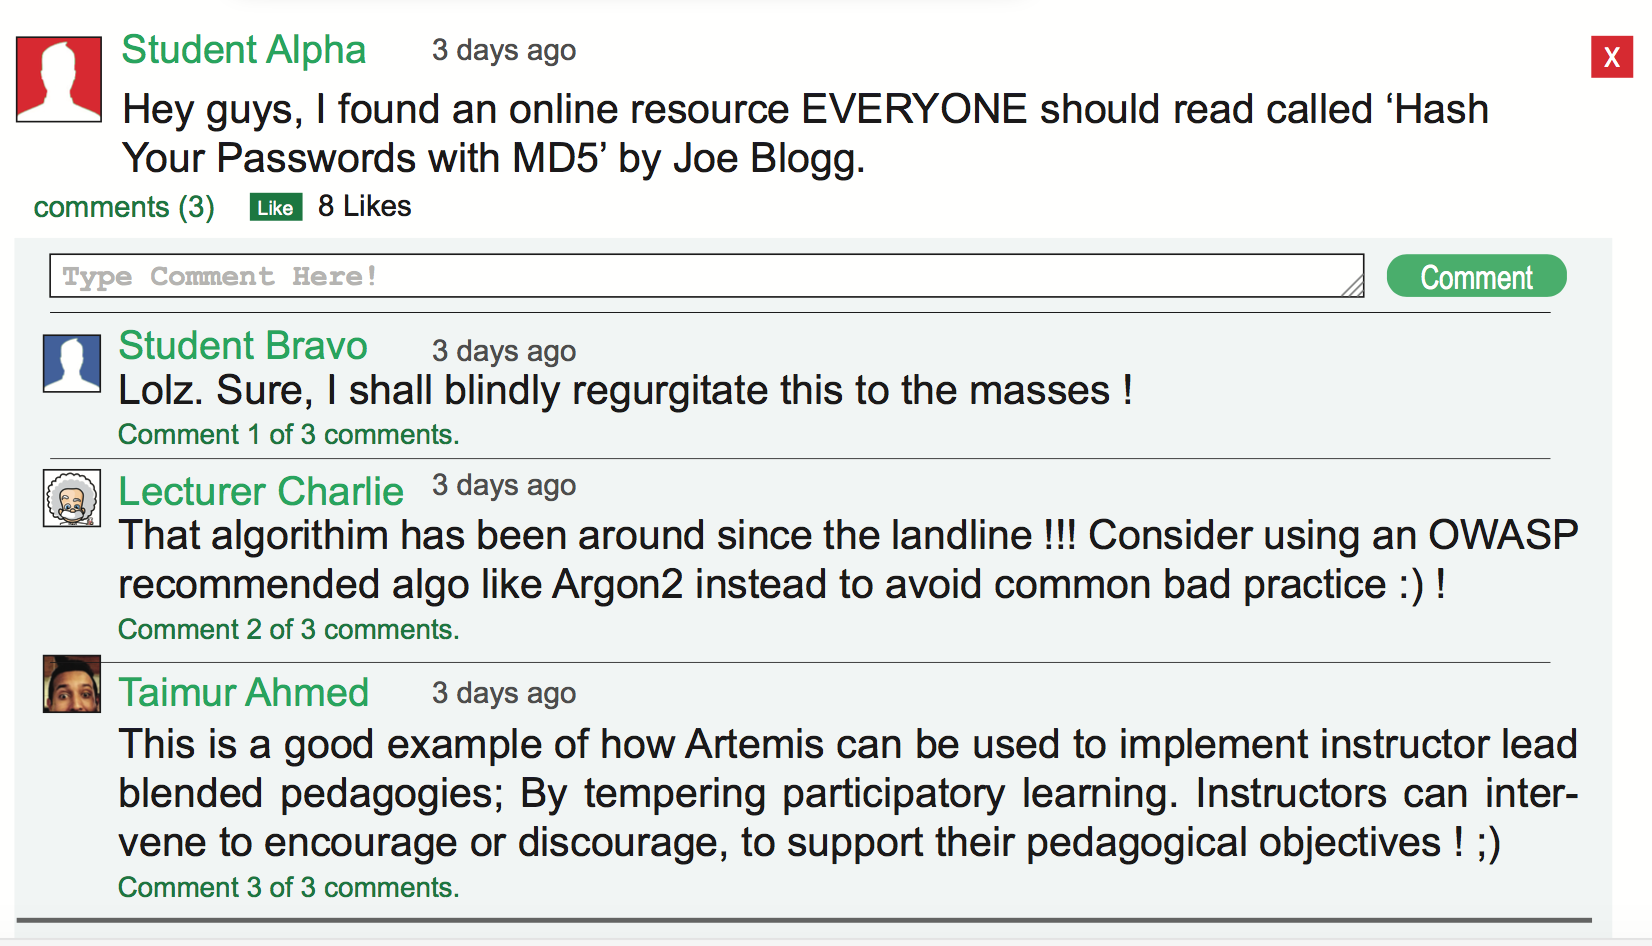
\includegraphics[scale=0.45,right]{chapters/chapter03/figures/comment.png}
        	\mycaption[Illustration of  Use Case, depicting possible adaptation of Participatory Learning Model to Proposed Social Network]{Illustration of  Use Case, depicting possible adaptation of Participatory Learning Model to Proposed Social Network}
        	\label{fig:UseCaseParticipatory}
        \end{figure}
        
        This possible use case (illustrated in previous figure) was also proposed during the focus group as well and the likelihood of it instructor intervention corroborated via course instructors. It was agreed upon by consensus that it is a reasonable assertion that when material is shared on Artemis it can easily be verified by other students, course instructors or teaching assistants via post \textit{likes} and \textit{comments}.
    
    \end{enumerate}
    
    \newpage
    \item \textbf{"Show that there's a real organization behind your site"} \cite{Fogg2002a}:
    
    A significant amount of development effort has been put into creating documentation for Artemis. Whilst the documentation has a wide and varied scope or purpose, it is essential to note that it indicates towards the existence of a professional team behind the project. A list of the documentation made readily accessible to Artemis users (i.e. always available in the application) is as follows:
    
    \begin{itemize}
    
        \item A \textbf{Wiki page} for Artemis so that users can find details about the project, underlying rationale, the programme specifications, legal modalities and information about the developers.
            \begin{figure}[H]
                \centering{ 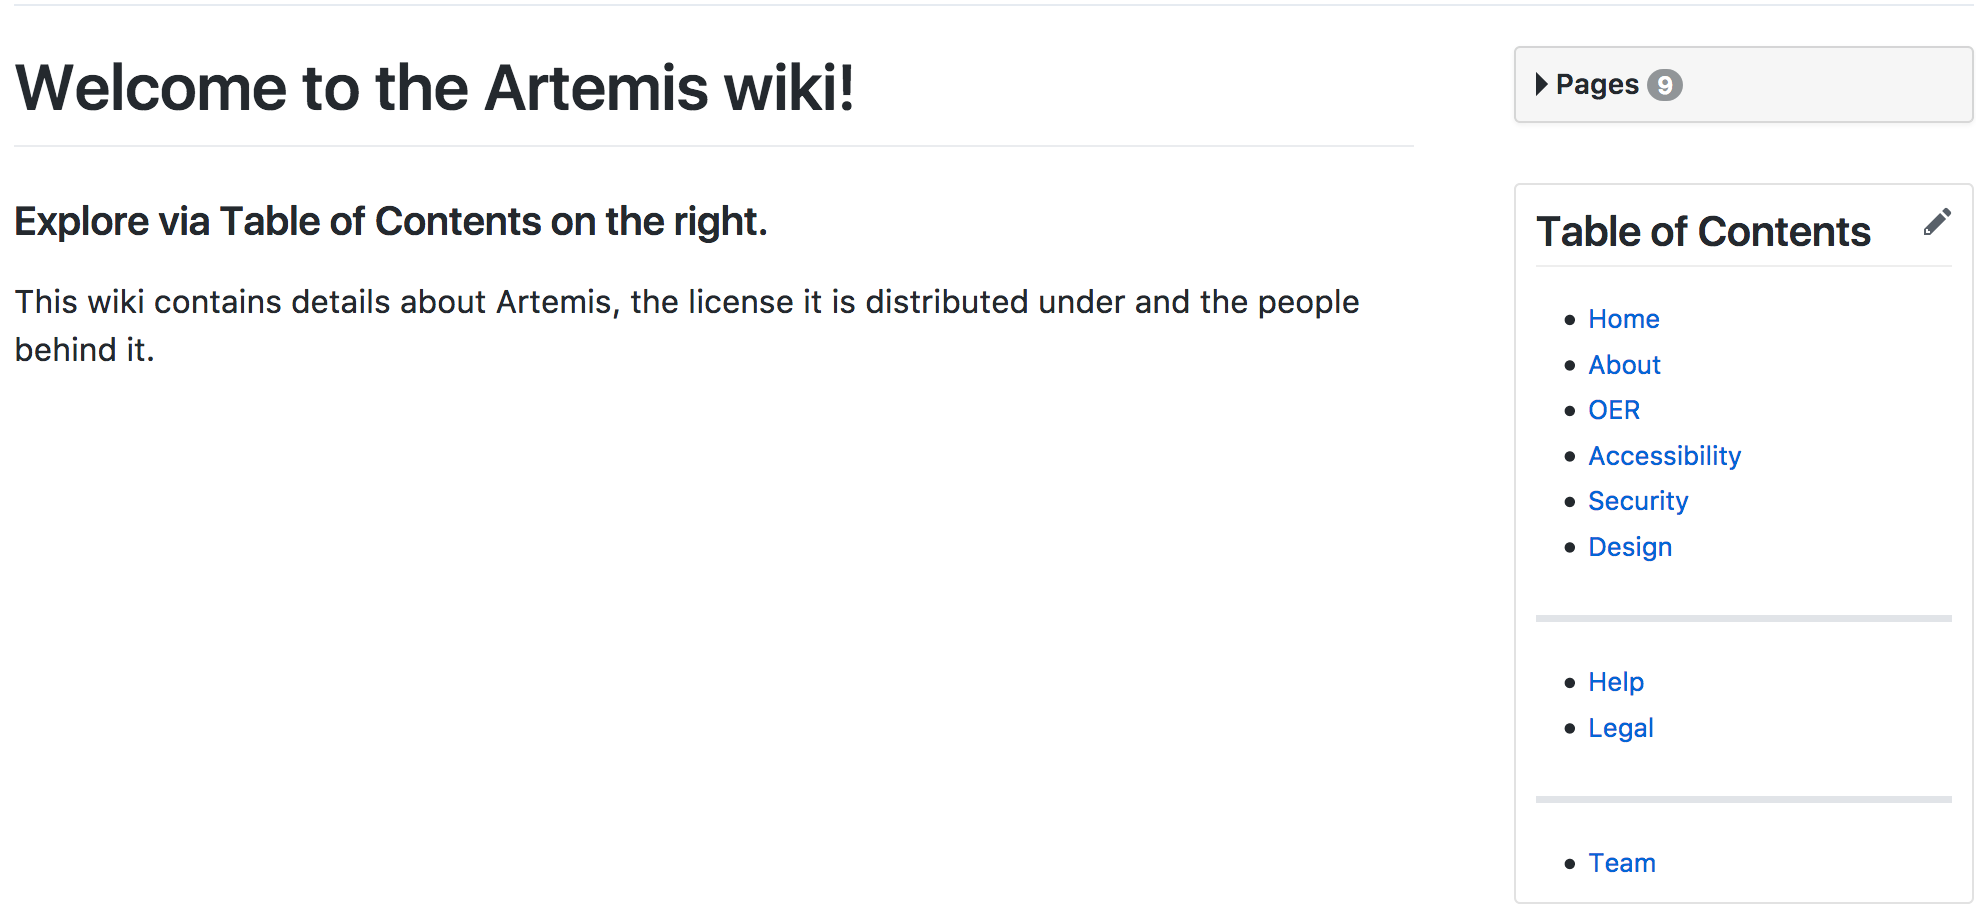
\includegraphics[scale=0.36]{chapters/chapter03/figures/Wiki.png}}
                \label{wiki}
                \caption{Artemis Wiki page. Available at: \url{https://github.com/TaimurAhmed/summerProject2017/wiki}}
            \end{figure}
            
        \item A \textbf{User Feedback and Bug Reporting page} on GitHub to so that users may report bugs and track issues. It also provides developers with a forum to discuss details of bugs, give feedback and reports as depicted in the following figure.
            \begin{figure}[H]
                \centering{ 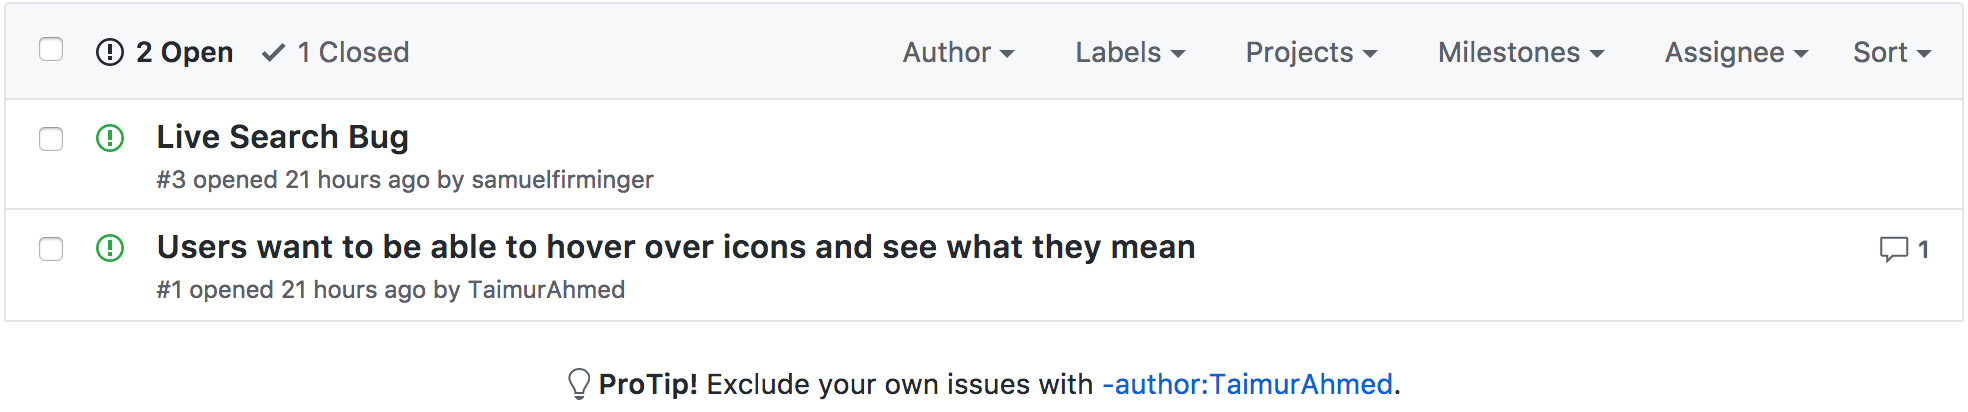
\includegraphics[scale=0.36]{chapters/chapter03/figures/bug.png}}
                \caption{Artemis Bug Report and Issue Tracking Page. Available at: \url{https://github.com/TaimurAhmed/summerProject2017/issues}}
            \end{figure}
        
        \newpage
        
        \item A \textbf{Developer Profile page} has been linked to the Wiki and can be accessed through the navbar.
            \begin{figure}[H]
                \centering{ 
\includegraphics[scale=0.36]{chapters/chapter03/figures/profile.png}}
                \label{developer}
                \caption{Developer Profile Page with contact details. Available at: \url{https://github.com/TaimurAhmed}}
            \end{figure}
        
        \item A \textbf{ReadMe markdown file} on GitHub for other developers. This is standard practice in most Open Source projects that want other developers to be able to understand and work on the project.
            \begin{figure}[H]
                \centering{ 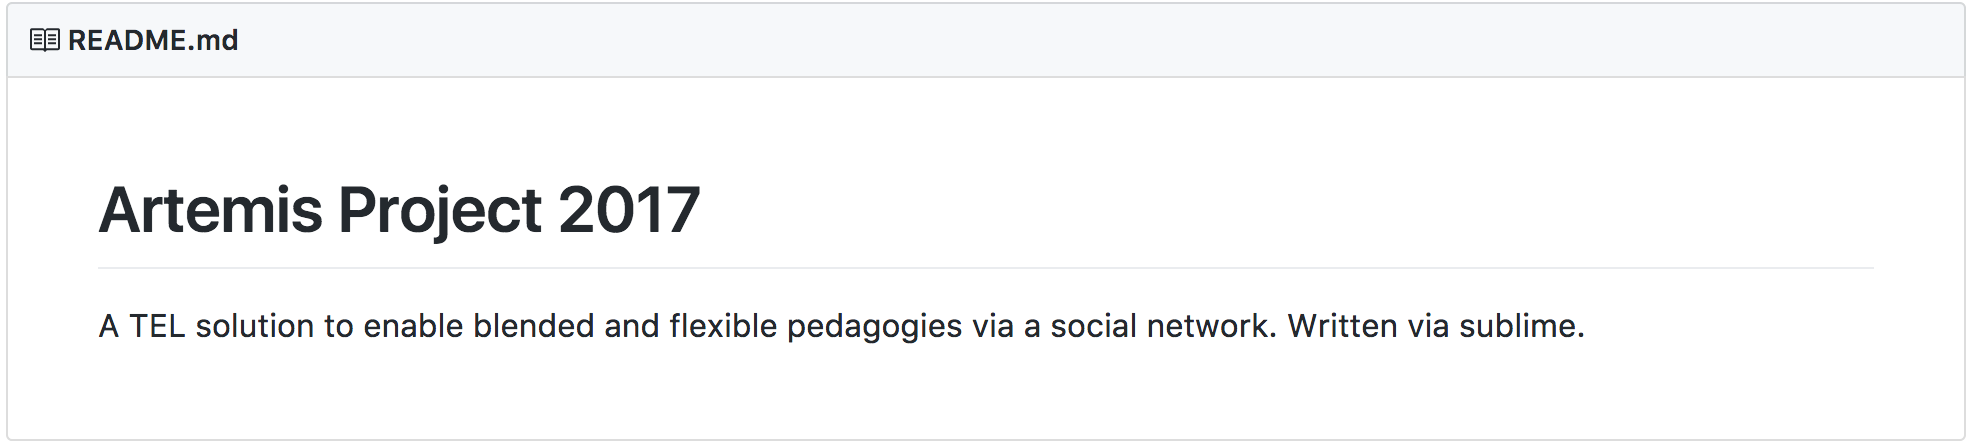
\includegraphics[scale=0.36]{chapters/chapter03/figures/readMe.png}}
                \caption{ReadMe Markdown File for Developers. Available at: \url{https://github.com/TaimurAhmed/summerProject2017}}
            \end{figure}
    \end{itemize}
    
    Furthermore UoB's offical favicons have been used (freely disseminated \cite{UniversityofBristola} and other default favicons were deprecated in favour of UoB's own logo \cite{UniversityofBristola} to further enhance user perception of a real organization. It is envisaged that if the tool is deployed in the future on UoB's in house servers this will further enhance this value as it will likely be disseminated via the organizations own web portal, giving users greater assurance within the relevant context (albeit Artemis is likely to have it's own domain name).


    \newpage    
    \item \textbf{"Highlight the expertise in your organization and in the content and services you provide."} \cite{Fogg2002a}:
    
   
   The Artemis Wiki as shown in the figure on \textbf{page \pageref{wiki}} has been used to highlight the technical aspects of Artemis e.g. the accessibility and security features behind Artemis via the content of the application. Furthermore the wiki is used to communicate the pedagogical rationale behind the project i.e. the design aspects and use cases. Effectively the wiki summarizes the technical and design features of the project for the benefit of users, so as to provide assurance in the expertise behind the project.
   
   The developer page which can also be accessed via Artemis can be used to highlight the expertise behind Artemis (ideally at the time of deployment an experienced team of developers will maintain the application and can reuse these links).
   
    \item \textbf{"Show that honest and trustworthy people stand behind your site"} \cite{Fogg2002a}:
    
    STPL recommends showing users that the people behind the web application are \textit{real} \cite{Fogg2002a}. This has been implemented in Artemis as follows:
    \begin{enumerate}
        \item Allowing for rich contextual data to be illustrated to the user when viewing other user's profiles i.e. users are able to determine that other profiles on the network either belong to fellow students or expert instructors.
        \item A separate page for biographical information of the developers as recommended by the STPL \cite{Fogg2002a} and illustrated on \textbf{page \pageref{developer}}.
        \item Making access to developer information and profiles available on all pages.
    \end{enumerate}
    
    \item \textbf{"Make it easy to contact you."} \cite{Fogg2002a}:
    
    This this can and has been done by simply adding developer contact details for bug reports, suggested improvements and feedback via the social networks to the UI i.e. the developers can be contacted via the click of a button in the nav bar of Artemis, which is accessible on every page of Artemis at all times. Furthermore detailed information is provided in the Wiki, ReadMe markdown, Bug and Error reporting page and developer's personal page to make it easy for users to contact the developer and learn more about the application.

    \item \textbf{"Design your site so it looks professional (or is appropriate for your purpose)"} \cite{Fogg2002a}:
    
    As recommended by STPL and implemented in this project , user acceptance testing was carried out to rigorously evaluate and subsequently refactor Artemis. User testers were intentionally encouraged to explore the application,  maliciously try to break it and undergo a series of Use Cases (See Appendix A1) unassisted. Whilst during the evaluation process the feedback was largely positive, a log of all issues was kept and all errors/user preferences were accounted for via code refactoring (Collated, identified and explained in a later chapter).

    \item \textbf{"Make your site easy to use"} \cite{Fogg2002a}:
    
    It was proposed during the focus group meeting with students that this can be done by seeking design inspiration from familiar social networks such as Facebook and Wikipedia, as users are likely to be familiar with the lay out and design of these sort of web applications\cite{Fogg2002a}. Furthermore the UI was evaluated and refactored as per user testing to enhance this aspect of user interaction and consideration  for assistive client side technologies such as screen readers or magnifiers was made with the use of ARIA (discussed in a later section of this chapter).
    
    \item \textbf{"Update your site's content often (at least show it's been reviewed recently)."} \cite{Fogg2002a}:
    
    Within the context of a Web 2.0 application that generates dynamically generated content contributed by the users, this should not necessarily be a problem. However after deployment the developer documentation that has been set up i.e. Wiki, Markdown file, Developer Page and Bug/Issue Report page, the relevant aspect of the project can be used to regularly update clients on recent releases and updates. This aspect is likely to be of more relevance after deployment and can only be anticipated preemptively. For the most part reasonable implementation is beyond the constraints of the project.
    
    \item \textbf{"Use restraint with any promotional content."} \cite{Fogg2002a}:
    
    As Artemis is not a commercial venture, this aspect of enhancing Web Credibility is easily addressed by using no promotional content.
    
    \item \textbf{"Avoid errors of all types, no matter how small they seem."} \cite{Fogg2002a}:
    
    The user evaluation testing was carried out without developer intervention and user testers were strongly encouraged to try and maliciously break and rigorously hack the program. This yielded valuable feedback used to refactor the code and will be discussed in a later chapter on evaluation and refactoring.
    
\end{enumerate}
\newpage


\section{Web Application Security}

With the transition of the world wide web from web-sites to web applications, i.e. the transition towards Web 2.0, a new host of security vulnerabilities moving away from traditional server side vulnerabilities towards new vectors such as vectors originating from client side have arisen \cite{Dayfdd2011}. Given the underlying importance of addressing common Web Application Security vulnerabilities \cite{Dayfdd2011} and it's negative impact on areas including but not limited to web credibility \cite{Fogg2002a,Fogg1999} that can affect the overall success and efficacy of the tool and even harm the users, this issue must be addressed for Artemis.

\subsection{OWASP}

An extensive review of web application security is desirable but beyond the reasonable constraints of this project. Therefore  utilising the \textit{Open Web Application Security Project (OWASP) Top 10} \cite{OWASP2017} for identifying common or important design vulnerabilities and mitigating them was  used during development, as a viable alternative achievable within the constraints of the project.

The Open Web Application Security Project is an online community  and  a respected  not-for-profit organisation which creates free to use articles, methodologies, documentation, tools, and technologies towards the benefit of web application security \cite{OWASP}. The organisation  annually releases research that identifies and underlines mitigation strategies for the \textit{"Ten Most Critical Web Application Security Risks"}\cite{OWASP2017} identified threat agents within the scope of qualitative benchmarks i.e. possible attack vectors, the prevalence and detectability of security vulnerabilities, the technical implications and the commercial/business implications.

The rationale behind these qualitative benchmarks to assist the quantification and ranking of security risks,  is illustrated as via the help of the following diagram which breaks a security vulnerability down into stages for classification and consideration:

% A single figure
\begin{figure}[H]
	\centering
	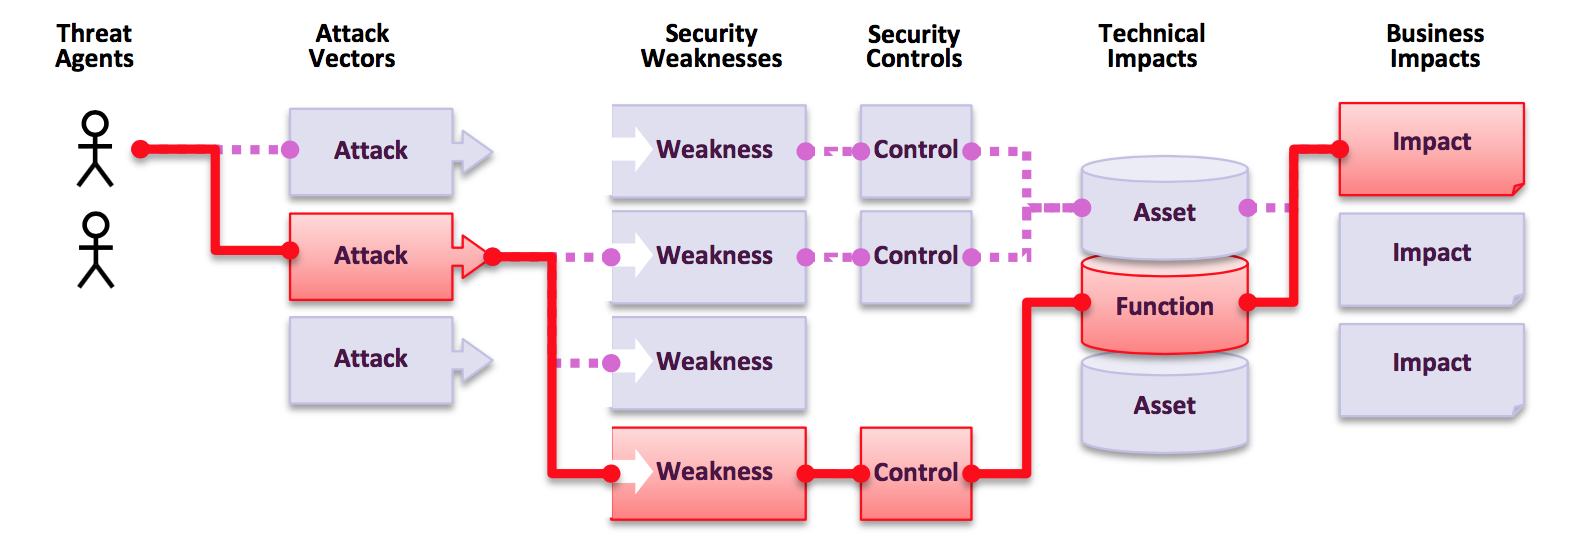
\includegraphics[scale=0.5]{figures/attack}
	\mycaption[Application Security - Consideration of Threat Agents]{Considerations of Threat Agents - . Figure reproduced from \cite{OWASP2017}.}
	\label{fig:Consideration of Threat Agents}
\end{figure}

The OWASP foundation reasons \cite{OWASP2017} that attackers or threat agents can exploit various modes of attack or \textit{attack vectors}, based on \textit{prevalence} and ease of \textit{detecting security weaknesses}/vulerabilities that can have a negative impact  within a generic technical or application specific commercial context \cite{OWASP2017}. Apart from application specific implications, the rest of these benchmarks can be classified based on the severity; which results in classification for the purpose of ranking the OWASP Top 10 vulnerabilities:

% A single figure
\begin{figure}[H]
	\centering
	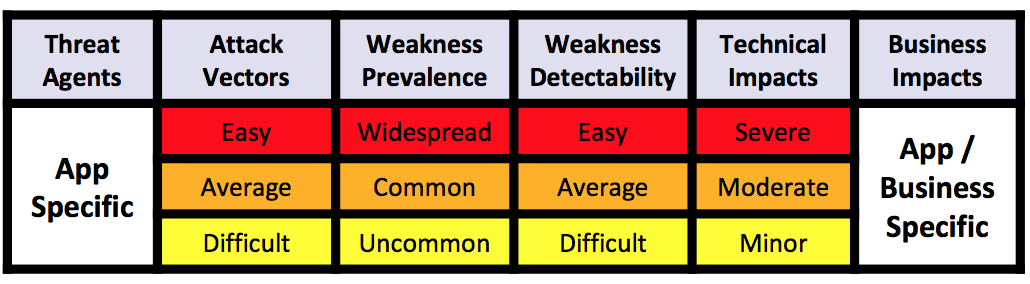
\includegraphics[scale=0.85]{figures/tabulation}
	\mycaption[OWASP Risk Rating Methodology]{OWASP Risk Rating Methodology - . Figure reproduced from \cite{OWASP2017}.}
	\label{fig:OWASP Risk Rating Methodology}
\end{figure}

Finally the risk rating methodology is used to compile an annual list of the most common, detectable and damaging security threats, along with mitigation strategies \cite{OWASP2017}. The proposed OWASP Top 10 for 2017, is effectively a mitigation strategy for this project that considers the likelihood and impact of security vulnerabilities. This seems to be a reasonable approach to security within the context of this project, as predicting attack vectors for every eventuality is not just futile but also undoubtedly unfeasible. Therefore within the context of the following attack vectors, Artemis has mitigated the risk as follows:

\begin{enumerate}
    \item \textbf{Injection}:
    
    \begin{figure}[H]
    	\centering
    	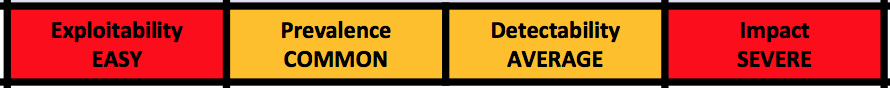
\includegraphics[scale=0.80]{figures/injection}
    	\mycaption[Injection Classification]{Injection Classification \cite{OWASP2017}.}
    	\label{injection}
    \end{figure}
    
    
    Injection vulnerabilities (particularly SQL injections) are the top vulnerability on the OWASP list \cite{OWASP2017}. As the \textbf{Figure \ref{injection}} illustrates, it is a prevalent and easily exploitable attack vector (as it is text based) which exploits interpretor syntax and can have a severe impact on an application e.g. MariaDB could be exploited by truncating all stored data or worse storing malicious data (The damage can be as severe as the hacker's imagination and ability).
    

    The most common cause of code injection i.e. SQL injection has been easily eliminated with via the use of prepared statements to interact with the MariaDB in Artemis. Otherwise known as a parameterised statement, a prepared statement is used to execute the same statement repeatedly with high efficiency and prevent SQL injection as per the PHP API\cite{PHP}. The use of prepared statements eliminates the possibility of SQL injection and avoid the pitfalls of relying on \textit{Escaping Strategy} (albiet as an extra layer of security Artemis does use PHP's native MySQLi escape methods, despite not actually being necessary in lieu of prepared statements), which can be notoriously hard to implement perfectly.
    
    To completely mitigate this attack vector within the context of Artemis, all user input is  sanitized via PHP's native \textit{strip\_tags} function. As per the PHP manual this sanitizes all PHP and HTML code into ordinary strings. Effectively the relevant interpreters have been insulated from user injected code and this risk has been almost eliminated in Artemis.
    
    In summary code injection has been prevented as follows:
    \begin{enumerate}
        \item Sanitizing User Input.
        \item Escaping User Input.
        \item Parameterised/Prepared Statements for storing sanitised and escaped user input into MariaDB.
    \end{enumerate}
    
    \begin{figure}[h]
    	\centering
    	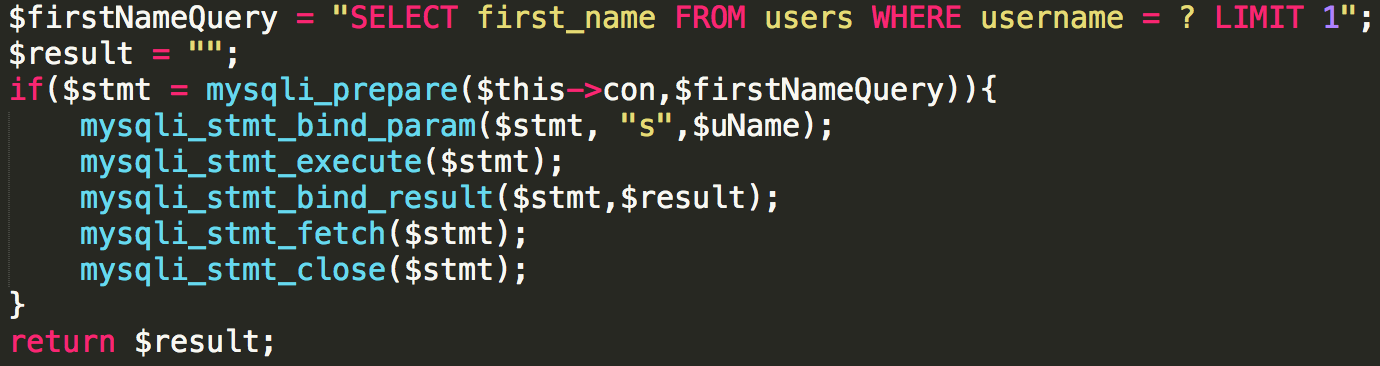
\includegraphics[scale=0.61,right]{chapters/chapter03/figures/preparedStmt.png}
    	\mycaption[Example Example Prepared Statementt]{Example Prepared Statement.}
    	\label{Example Prepared Statement}
    \end{figure}
    

    \item \textbf{Broken Authentication and Session Management}:
    
    \begin{figure}[h]
    	\centering
    	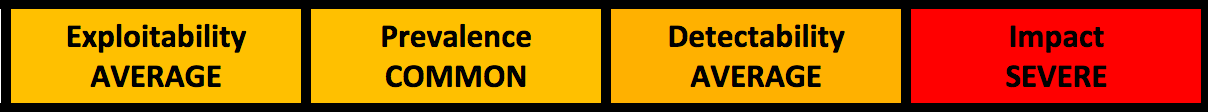
\includegraphics[scale=0.55,center]{chapters/chapter03/figures/xss.png}
    	\mycaption[Broken Authentication and Session Management Classification]{Broken Authentication and Session Management Classification \cite{OWASP2017}.}
    	\label{Broken Authentication and Session Management Classification}
    \end{figure}
    
    
    As the \textbf{Figure \ref{XSS Classification}} illustrates OWASP found that authentication and/or session management functionality are often implemented incorrectly \cite{OWASP2017}. Effectively this could allow malicious attackers to compromise passwords, keys, or session tokens, and other flaws via assuming a victim's identity on the social network \cite{OWASP2017}, making the potential commercial and technical implications severe.
    
    OWASP PHP Security project finds that the PHP's default session facility is safe and generates a session id that is sufficiently random \cite{OWASPa}. However the project does recommend steps to prevent common attack vectors within this category such as session hijacking. Therefore whilst using PHP's session facilities the additional considerations have been addressed as follows:
    

    \begin{enumerate}
        \item \textbf{Session Hijacking}: 
        \begin{enumerate}
            \item Session Fixation\cite{OWASPa} \hl{and} Rolling Session ID's: After a successful user login and with each page visit the session id has been regenerated using the PHP function \textit{session\_regenerate\_id}. Effectively each page visit invalidates the last session id reducing the risk of compromise due to a hijacked session.
            \item Invalidate Session ID: Incorrect session ID's are invalidated and users are forcefully redirected to the application log in page, regardless of which page they are on via the use of header.php.
            \item Session Expiration: Sessions are expired after 30 seconds of inactivity as per OWASP recommendations, using the PHP function \textit{session\_set\_cookie\_params} to configure session cookies and server side management.
        \end{enumerate}
        \item \textbf{Cookie Management}:
        OWASP \cite{OWASPa} recommends standard good security practices such as not serializing cookie data (due to an increased scope of security concerns) or storing sensitive data in a cookie (which can easily be accessed by a hacker or even the user themselves).  These have been incorporated in Artemis's design.
        \begin{enumerate}
            \item Cookie Parameters: The \textit{cookie\_params} function has been used to secure the cookie settings for artemis. This involves:
                \begin{itemize}
                    \item Setting a cookie lifetime (30 seconds).
                    \item Path on the domain where the cookie will work; Currently set to work on the entire domain but will need to be reconfigured during production or actual deployment.
                    \item Cookie domain, currently local host but will need to be reconfigured as reasonable at the time of deployment.
                    \item Secure connection transport protocol; See below for details on SSL.
                    \item Enabling HTTP only session cookies;See below for details.
                \end{itemize}
                Clearly not all of cookie settings security features can  be factored in during development by default as some of them rely on the existence of an actual domain name i.e.SSL,HTTP/HTTPS, domains and path. A self signed certificate in these instances to enable an HTTPS connection and SSL is at best a half measure and would ultimately need to be replaced once an actual domain is secured. Therefore clear and explicit disclosure has been made in developer documents regarding re-factoring at the time of deployment and within the source code itself; Toggling these security features is as simple as changing a boolean value, which is deemed not unreasonably onerous for anyone adapting the open source program as long as it is clearly disclosed. Relevant disclosure have been made in the source code (See figure \ref{ProductionCookieMessage}), Wiki and Markdown File of Artemis.
                \begin{figure}[h]
                	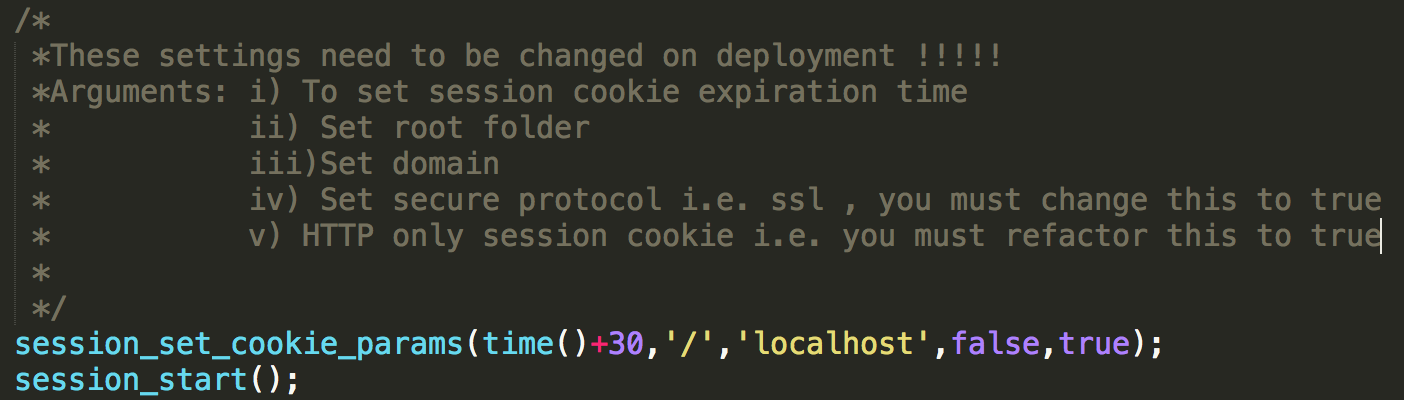
\includegraphics[scale=0.55,right]{chapters/chapter03/figures/secureSession.png}
                	\mycaption[Source Code Comment for Cookie Params during Production]{Source Code Comment for Cookie Params during Production.}
                	\label{ProductionCookieMessage}
                \end{figure}
                            
        \end{enumerate}
    \end{enumerate}

    \item \textbf{Cross Site Scripting (XSS)}:
    
    \begin{figure}[h]
    	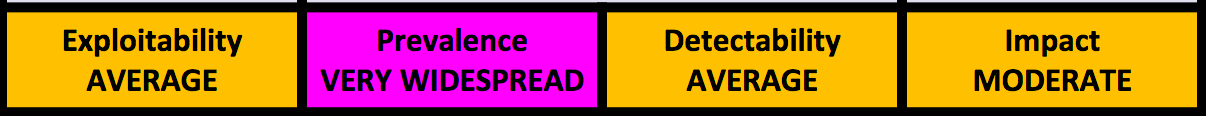
\includegraphics[scale=0.55,center]{chapters/chapter03/figures/XSSClassification.png}
    	\mycaption[Source Code Comment for Cookie Params during Production]{Source Code Comment for Cookie Params during Production.}
    	\label{XSSclassification}
    \end{figure}
    
    XSS vulnerabilities are notoriously widespread, easy attack vectors to exploit and  usually client's bear the brunt of the fallout \cite{OWASP2017} as illustrated by \textbf{figure \ref{XSSclassification}}. XSS includes the inclusion of untrusted data (malicious text based attack scripts)in a new web page without proper validation or escaping \cite{OWASP2017}; particularly problematic with client side browsers and JS. Depending on the application use case XSS mitigation can take many forms. As HTML and PHP tags are  unnecessary user input in Artemis, this risk has been completely mitigated by using the sanitisation strategy mentioned during the mitigation of code injection. The user input sanitisation strategy which relies on stripping HTML, PHP tags and   converting HTML entities  to ordinary strings has the added advantage of completely mitigating XSS.
    
    \textbf{Security Extension: Self XSS}:
    While OWASP doesn't specifically identify guarding against Self XSS  a variant of the XSS attack, which makes use of social engineering attack vectors\cite{FaceBook}; An inspection of the  the client side code for FaceBook and Google Hangouts reveals that mainstream social networks such as the aforementioned warn users against self XSS attacks. In the past FaceBook adopted an approach that would warn the user of Self XSS and disable the client side console; however for obvious reasons this was deemed problematic and exploitable by major browser vendors and prevented accordingly \cite{StackO}. These days FaceBook has adopted the approach illustrated in \textbf{Figure \ref{faceBookSelfXSS}}, so as to mitigate the possibility of social engineering attack vectors.
    
    \begin{figure}[h]
    	\centering
    	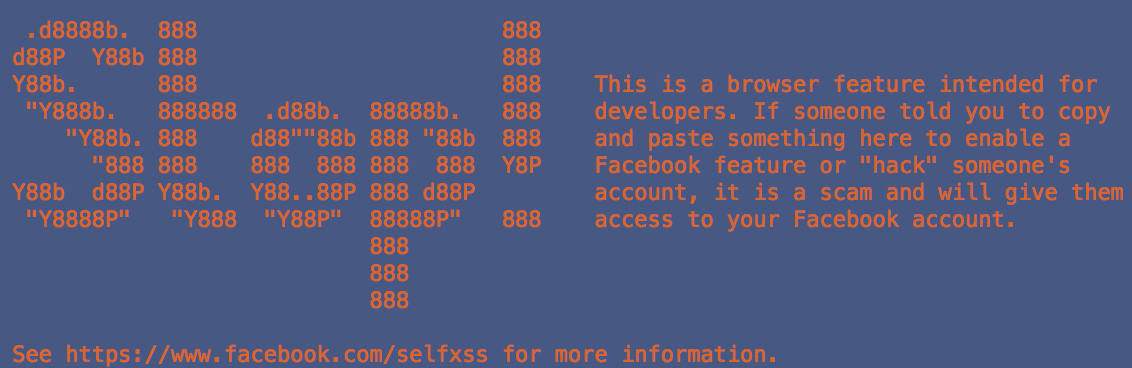
\includegraphics[scale=0.75,right]{chapters/chapter03/figures/faceBook.png}
    	\mycaption[FaceBook Self XSS Warning]{FaceBook Self XSS warning in browser console.}
    	\label{faceBookSelfXSS}
    \end{figure}
    
    As the figure above illustrates this a simple console message, meant to grab the attention of the client; should they try to access developer tools in their browser whilst using the FaceBook application. As this idea is reasonably simple to implement it was added to Artemis. However in an effort to extend the purpose behind this message a decision was made to try an enhance the efficacy of this mitigation strategy by using CSS3  to highlight the attention and grab the user's attention before they attempt self XSS.
    
    \begin{figure}[h]
    	\centering
    	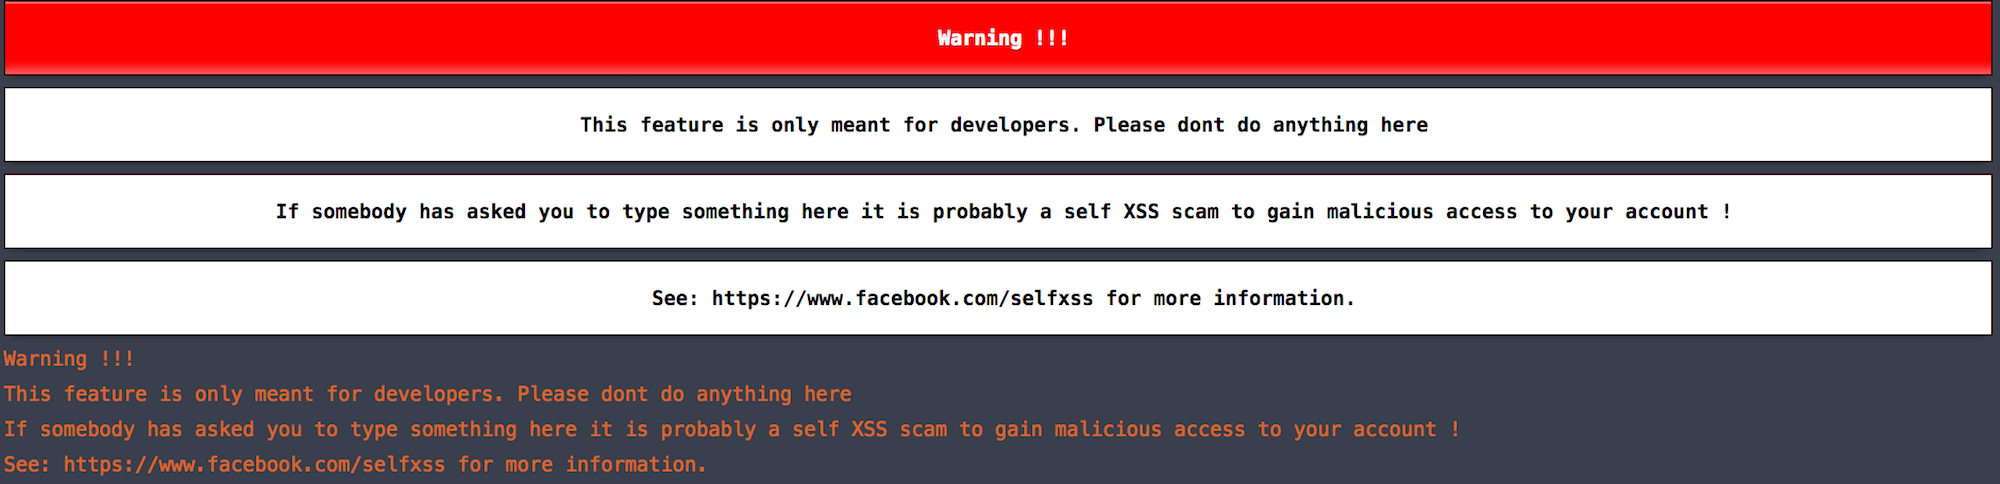
\includegraphics[scale=0.44,right]{chapters/chapter03/figures/ArtemisXSS.png}
    	\mycaption[Artemis Self XSS Warning]{Artemis Self XSS warning via browser console.}
    	\label{ArtemisSelfXSS}
    \end{figure}   
    
    
    
    \newpage
    
    \item \textbf{Broken Access Control}:
    
    \begin{figure}[h]
    	\centering
    	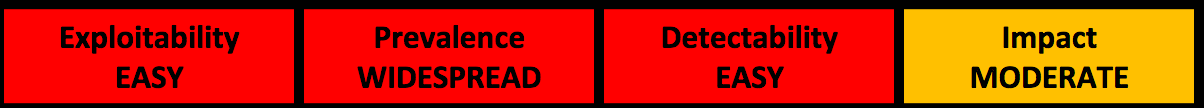
\includegraphics[scale=0.5,center]{chapters/chapter03/figures/brokenAccess.png}
    	\mycaption[Broken Access Control Classification]{Broken Access Control Classification.}
    	\label{Broken Access Control}
    \end{figure}
    
    Broken or non-existant access control can give third parties access to sensitive information or worse allow access to the settings page on Artemis and allow malicious users to hijack an account.
    
    A White Listing or Black Listing strategy was considered for the purposes of Artemis, but was deemed onerous for implementing within the context of a dynamically generated application with it's straightforward design. Instead Artemis makes use of server side and database logic to serve various access control relevant features such as personal messages, comments, newsfeed, bio etc. Therefore it is realistically not possible (assuming no human error) to view information that a person does not have access to, if the server side DB logic does not concur. E.g. If a person tries to access the newsfeed of a person they are not friends with via \textit{direct object reference}, it is not possible as server side logic will only serve them the information if the database corroborates that the two users are friends i.e. if they are not friends they will only be served a page where they can \textit{friendship request} the relevant user.
    
    During user evaluation some feedback was received regarding blocking malicious users due to ethical issues such as cyber bullying. This will be discussed in the concluding chapters.
    
    \item \textbf{Security Misconfiguration}:
    
    \begin{figure}[h]
    	\centering
    	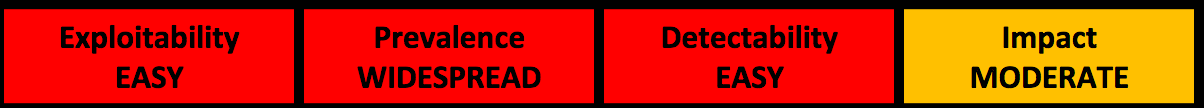
\includegraphics[scale=0.5,center]{chapters/chapter03/figures/brokenAccess.png}
    	\mycaption[Security Misconfiguration Classification]{Security Misconfiguration Classification}
    	\label{Security Misconfiguration}
    \end{figure}
    
    Security configuration refers to basic hardening exercises at the time of production, which if forgone can lead to application specific vulnerabilities \cite{OWASP2017}. Therefore Artemis adopted OWASP's recommendations for configuring and hardening the application.
    
    As per OWASP \cite{OWASPa} PHP is by default an insecure language for deployment. The reason for this is that PHP needs to be reconfigured to switch from development mode to settings more suitable for deployment e.g. by default DB errors will lead to a PHP application leaking sensitive server and directory information which a hacker can use to probe an application and discover vulnerabilities. The file responsible for configuring php is known as \textit{php.ini} or the \textit{configuration file}\cite{PHPa}.
    
    The configuration file allows for useful settings to be turned on such as detailed error messages during development. However what is an asset during development is usually a major liability during production or deployment. Therefore a php.ini file has been shared in the project; solely for the purpose of deployment as opposed to development.
    
    The configuration file has been broken up as follows and is explained accordingly \cite{OWASPa}:
    \begin{itemize}
        \item \textbf{PHP Error Handling}\cite{OWASPb}: OWASP's PHP project recommends the following settings  illustrated below. The underlying rationale here is to turn off features such as compiler warnings that may reveal sensitive information about the source code of the program. Whilst these settings are helpful during development they are not suitable from a security perspective during production.
            \begin{figure}[H]
            	\centering
            	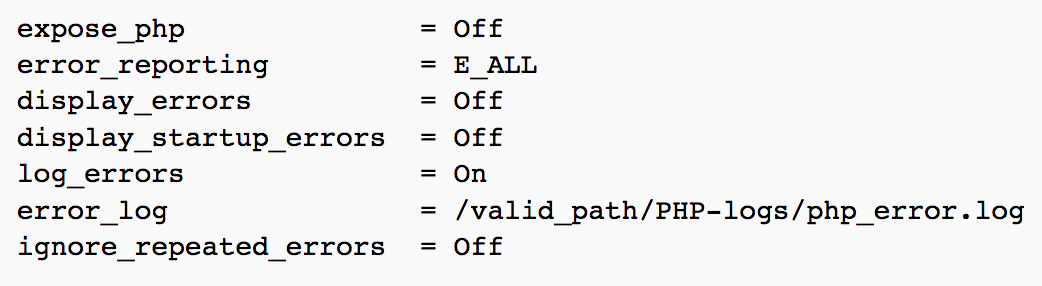
\includegraphics[scale=0.44,center]{chapters/chapter03/figures/errorPHP.png}
            	\mycaption[PHP Error Handling Configuration]{PHP Error Handling Configuration}
            	\label{PHPError}
            \end{figure}   

        \item \textbf{PHP General Settings}\cite{OWASPb}: URL routing and default directory setup is usually vulnerable in PHP. The following settings are good practice and prevent scenarios such as easy escalation of local file inclusion to remote file inclusion and explicitly setting the document root folder.
        
            \begin{figure}[H]
            	\centering
            	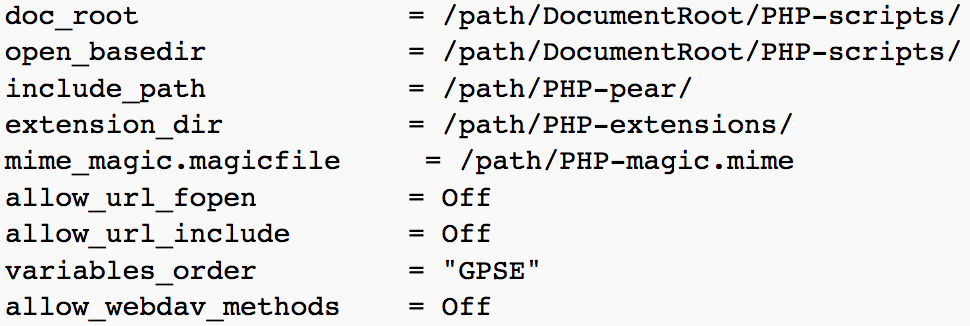
\includegraphics[scale=0.44,center]{chapters/chapter03/figures/generalPHP.png}
            	\mycaption[PHP General Configuration]{PHP General Configuration}
            	\label{PHPGeneral}
            \end{figure}   
        
    
        \item \textbf{PHP Executable Handling\cite{OWASPb}: OWASP} \cite{OWASPb} explicitly identified the following as extremely insecure function in PHP which need to be turned off unless explicitly necessary, as they can be exploited be clearly used by hackers to create havoc. As Artemis does not use them they are deemed unnecessary and therefore disabled:
            
            \begin{figure}[H]
            	\centering
            	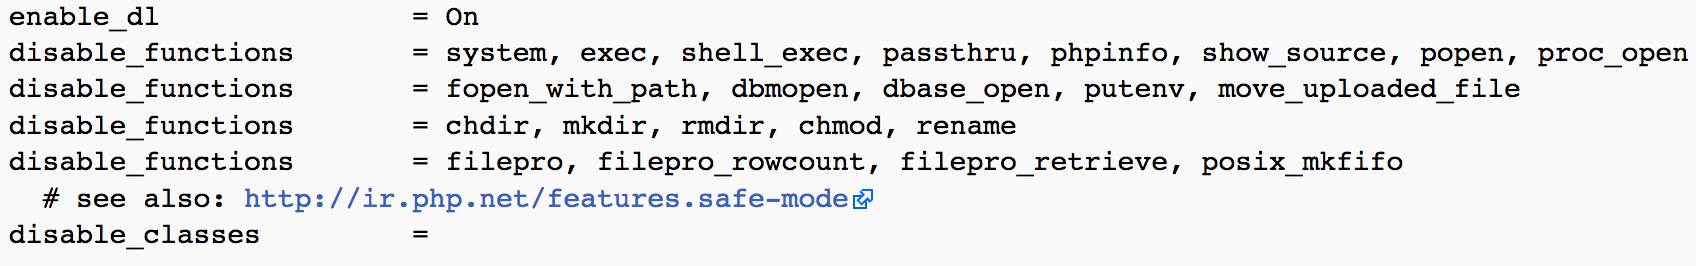
\includegraphics[scale=0.44,center]{chapters/chapter03/figures/execPHP.png}
            	\mycaption[PHP Executable Handling Configuration]{PHP Executable Handling Configuration}
            	\label{PHPExec}
            \end{figure}

        \item \textbf{PHP Session Handling}\cite{OWASPb}:
        
        OWASP recommends reconfiguring session handling\cite{OWASPb} as good practice recommended by security professionals; e.g. by renaming session names to deter script based attacks. These recommendations have been summarized as follows:

            \begin{figure}[H]
            	\centering
            	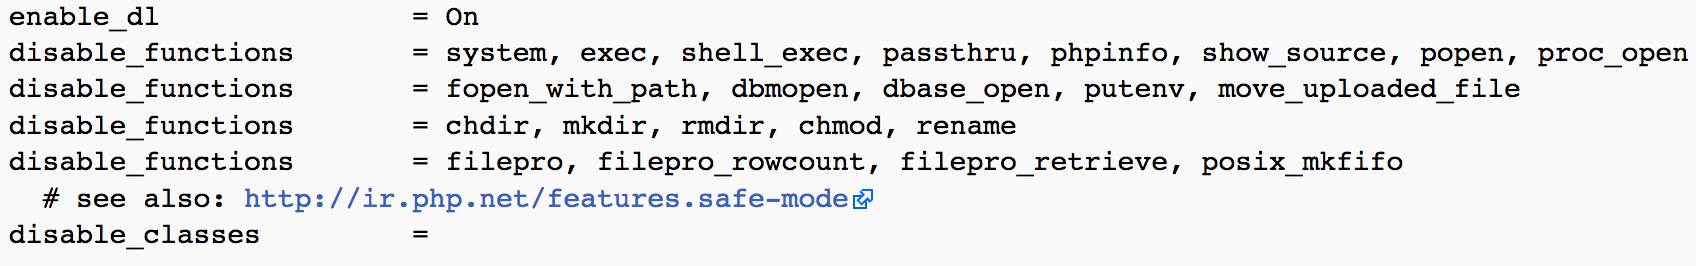
\includegraphics[scale=0.44,center]{chapters/chapter03/figures/execPHP.png}
            	\mycaption[PHP Session Handling Configuration]{PHP Session Handling Configuration}
            	\label{PHPSess}
            \end{figure}  
            
        \item \textbf{Database Configuration}\cite{OWASPb}:
        
        There are two main database configurations for MariaDB that need to be highlighted. First of the root user's password has not been set which is \textbf{bad security} practice. However this is justified by the fact that Artemis is in development and not yet ready for production. Therefore relevant disclosure has been made in the developer documentation to alert possible parties interested in forking the project to set there own DB password and admin user settings.
        
        Furthermore as per OWASP recommendations UTF-8 has been used as the database and application charset to avoid unpredictable security outliers \cite{OWASPa,OWASPb} that might not have been mitigated for.
        

    \end{itemize}
    
    
    
    
    
    
    \item \textbf{Sensitive Data Exposure}:

    \begin{figure}[h]
    	\centering
    	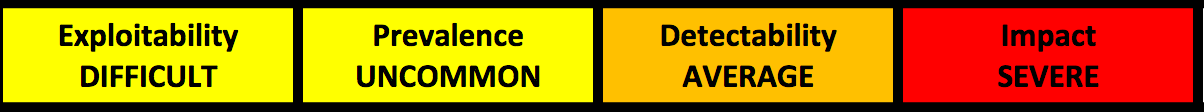
\includegraphics[scale=0.5,center]{chapters/chapter03/figures/sensitive.png}
    	\mycaption[Sensitive Data Exposure Classification]{Sensitive Data Exposure Classification}
    	\label{Sensitive Data Exposure}
    \end{figure}
    
    Within the context of Artemis this attack vector refers to leaked passwords that have not been correctly encrypted. It is worth noting that this seemed particularly problematic in the PHP community where many respected tutorials and forums recommended hashing with MDA5  as opposed to encryption with a modern algorithm.
    
    OWASP strongly recommends against encrypting sensitive data with MDA5, as it is almost trivial to decry pt \cite{OWASPc}. It recommends the usage of other modern algorithms ideally Argon2 which uses a modern encryption algorithm \cite{OWASPc}. However Argon2 is not yet available in PHP's native functions. Whilst it has been proposed for release in upcoming versions (due after the submission of this project), there are other encryption algorithms available which are also approved by OWASP i.e. Bcrypt. Therefore Artemis has encrypts it's passwords with Bcrypt but recommends switching to Argon2 as soon as it is available in the new PHP release. This approach is deemed safer than using an external library from a relatively unknown source. It is also worth adding that all encryption algorithms should and have been \textit{salted}.
    
    Further consideration has been given to data encryption by using the default hashing algorithm within the PHP library; i.e. it is regularly updated to increase the hash length or the algorithm (as per the PHP manual \cite{PHPc}). Therefore consideration within the database has been made by allowing for a recommended 255 characters.
    
    Finally the default salt has been used as per PHP's own recommendations and the algorithm cost for the salt has been set at minimum of default 10 as per the PHP manual. However the following method has been provided for developers to use during production; In case their server allows for a higher cost (without it being unnecessarily onerous) by calculating an appropriate cost using native PHP function:


    \begin{figure}[h]
    	\centering
    	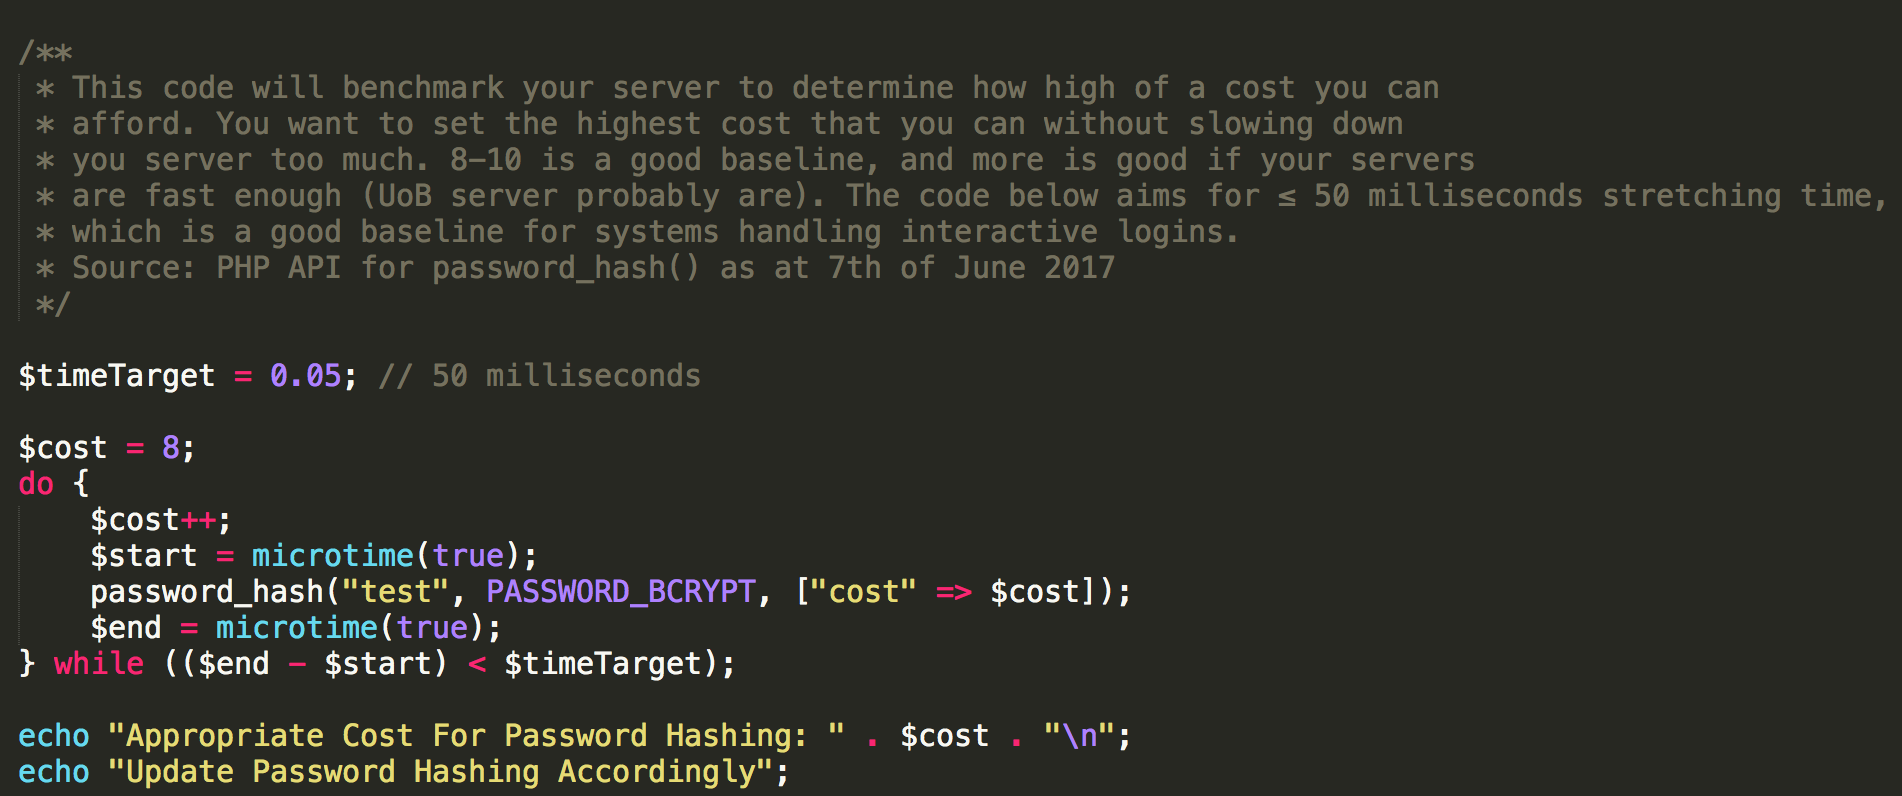
\includegraphics[scale=0.4,center]{chapters/chapter03/figures/cost.png}
    	\mycaption[Method for Calculating Salt Cost]{Method for Calculating Salt Cost}
    	\label{Salth}
    \end{figure}
    
    
    
    
    
    \newpage
    
    \item \textbf{Insufficient Attack Protection}:
    
    \begin{figure}[h]
    	\centering
    	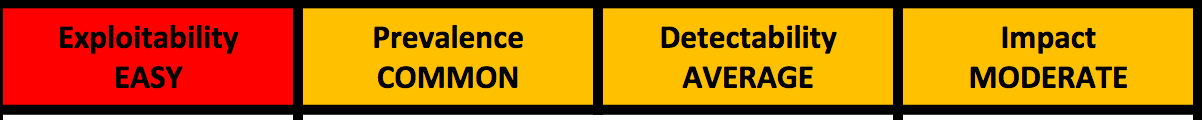
\includegraphics[scale=0.5,center]{chapters/chapter03/figures/Attack.png}
    	\mycaption[Insufficient Attack Protection Classification]{Insufficient Attack Protection Classification}
    	\label{Attack}
    \end{figure}
    
    This refers to app vulnerabilities such as APIs which lack the basic ability to detect, prevent, and respond to both manual and automated attacks \cite{OWASP2017}. The problem with mitigating this aspect of web security is two fold; it is generally reactive and specific to production. Therefore it has been largely ignored during this project and the onus of sufficient attack protection has been left on those adopting the technology during production.
    
    \item \textbf{Cross Site Request Forgery (CSRF)}:
    
    \begin{figure}[h]
    	\centering
    	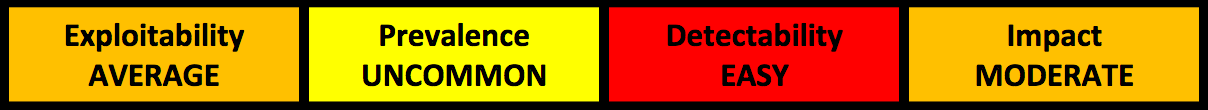
\includegraphics[scale=0.5,center]{chapters/chapter03/figures/csrfClass.png}
    	\mycaption[CSRF Classification]{CSRF Classification}
    	\label{CSRF}
    \end{figure}
    

    
    
    A CSRF attack forces a logged-on victim browser to send a forged HTTP request, including the victim\textquotesingle s session cookie and any other automatically included authentication information, to a vulnerable web application \cite{OWASP2017}. Already introduced mitigation strategies for other aspects such as cookie management, session hijacking, injection and sanitisation reduce the possibility of this attack vector as it usually relies on social engineering and/or malicious code.
    
    However as CSRF attack usually misuses a web application to create undesired affects, special emphasis has been  and should be \cite{OWASPa} placed on particularly sensitive data such as account settings which involve changing the password (the password is encrypted data and therefore of high value). In this instance the \textit{Google Recaptcha V2 API} was utilised to add an extra layer of security to prevent CSRF. Furthermore the optional IP tracking argument has been used to deploy the Recaptcha to track malicious activities.
    
    \newpage
    The implementation  of ReCaptcha on Artemis pages is illustrated as follows:
  
    \begin{figure}[h]
    	\centering
    	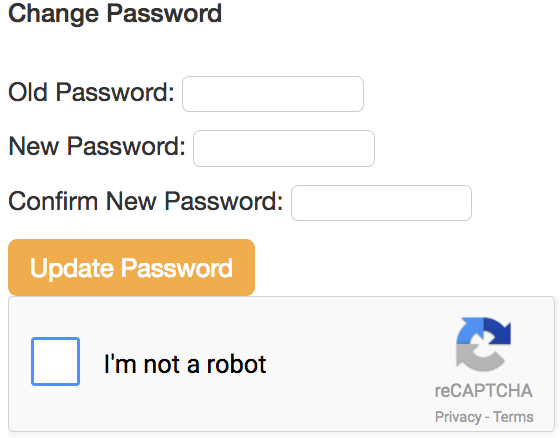
\includegraphics[scale=0.44,center]{chapters/chapter03/figures/captchaGoogle.png}
    	\mycaption[Google ReCaptcha]{Google ReCaptcha. Request on Artemis Accounts Settings Page.}
    	\label{googleRecaptcha}
    \end{figure}  
    
=    
    \begin{figure}[h]
    	\centering
    	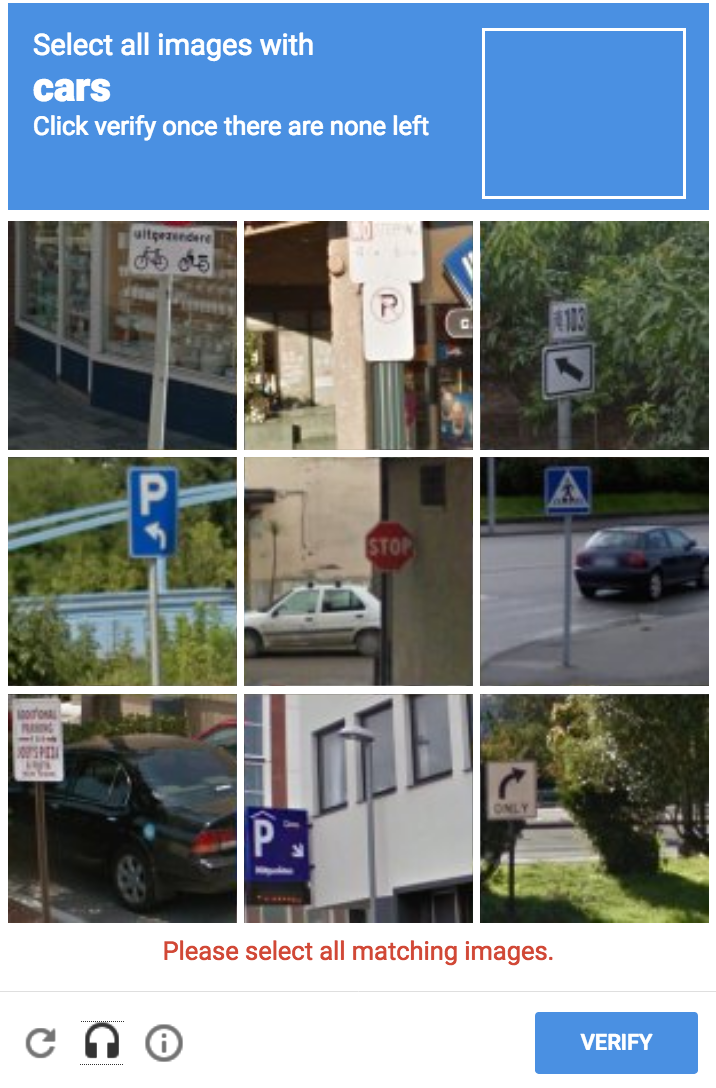
\includegraphics[scale=0.44,center]{chapters/chapter03/figures/verifyGoogle.png}
        \mycaption[Google ReCaptcha]{Google ReCaptcha Test on Artemis Password Settings Page .}
        \label{ArtemisSelfXSS}
    \end{figure}  
    

    
    
    \newpage
    \item \textbf{Using Components with Known Vulnerabilities}:
    
    \begin{figure}[h]
    	\centering
    	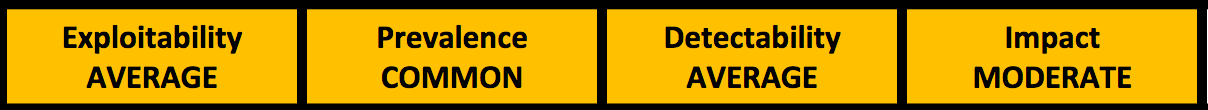
\includegraphics[scale=0.5,center]{chapters/chapter03/figures/components.png}
    	\mycaption[Vulnerable Component Threat Classification]{Vulnerable Component Threat Classification}
    	\label{vulnerable}
    \end{figure}
    
    Components, such as libraries, frameworks, and other software modules, which run with the same privileges as the application pose the threat of potential attack vectors if a vulnerable component is exploited  \cite{OWASP2017}. However nearly all of the strategies for this aspect of security are iterative and almost completely reactive as opposed to practive. Therefore the onus has been placed on development during production and excluded from the scope of the project.
    
    Reasonable attempts have been made by researching external components before using them and making sure that said components are popular in the open source community and therefore the chances of outstanding security issues is low.
    
    \item \textbf{Underprotected API's}:
    
    \begin{figure}[h]
    	\centering
    	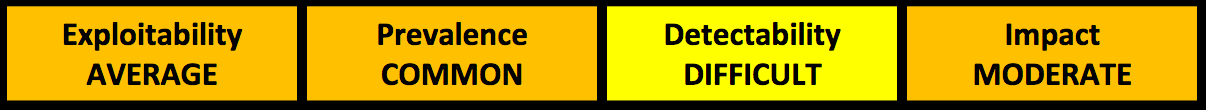
\includegraphics[scale=0.5,center]{chapters/chapter03/figures/api.png}
    	\mycaption[Underprotected API Threat Classification]{Underprotected API Threat Classification}
    	\label{Underprotected API}
    \end{figure}

        
    Modern applications often involve rich client side applications and APIs, such as JavaScript in the browser and mobile apps, that connect to an API of some kind (SOAP/XML, REST/JSON, RPC, etc)\cite{OWASP2017}. These APIs are often unprotected and contain numerous vulnerabilities" \cite{OWASP2017}.
    
    However as with vulnerable components, vulnerable API's need to be a part of an iterative and reactive strategy during production. Therefore most mitigation strategies are beyond the scope of this project. However attempts have been made to at least study the PHP API's vulnerabilities by refering to the PHP security project  for the development of Artemis and the resulting security mitigation strategy has been largely inspired by it.
    
\end{enumerate}



\newpage
\section{Accessibility}

Accessibility within the context of Artemis refers to interaction with both those who use assistive client side technologies such as screen readers or magnifiers \cite{MozillaDeveloperNetworka} and those who do not e.g. users with weak or impaired eyesight \cite{W3Cb}. To quote the Mozilla Developer Network on the matter of accessibility, \say{\textit{The Web is fundamentally designed to work for all people, whatever their hardware, software, language, culture, location, or physical or mental ability. When the Web meets this goal, it is accessible to people with a diverse range of hearing, movement, sight, and cognitive ability} \cite{MozillaDeveloperNetworka}}. Beyond the aforementioned lofty ideal\textquotesingle s there is a strong underlying theoretical and commercial rationale for designing Artemis, so that it is accessible:

\begin{enumerate}

    \item As proposed; Artemis is a Web2.0 solution i.e. it generates dynamic content. In the past statically generated content had the advantage of being easy to access via assistive technologies such as screenreaders, however an application that relies on complex dynamically generated content will almost certainly be inaccessible to assistive technology if considerations are not made for client side device interaction \cite{MozillaDeveloperNetwork}. If a sample of users can not access a technology such as Artemis, it stands to reason that Artemis is a \textbf{commercial and pedagogical failure} for the relevant audience.
    
    Accessibility as a design value \textbf{supports and ties together underlying design} principles and rationale such as Web Credibility and Pedagogy. It can be argued that the former is enhanced by creating \textit{persuasive technology} via enhancing the perception of professionalism and skil; The latter benefits by allowing instructors to interact with all students and conveniently apply one single pedagogy for everyone.
    
    \item Meetings with the TELED department bought to light that it is not uncommon at the UoB for accessibility issues to be reported when TEL solutions or even basic web pages have been deployed in the past. Albiet while was revealed that whilst most commercial strategies are reactive and subject to user feedback by necessity of the virtue that humans disabilities vary, it does not imply that proactive development strategies to improve client side technology interaction can not be used at the point of project conception\cite{W3C}.
    
    \item Beyond ethical,commercial and pedagogical rationale; Accessibility is a growing legal concern i.e. within some jurisdictions accesible access to technology and products is enforced by law  \cite{Network}.
    

    
\end{enumerate}

It is recognized that accessibility issues can cover a wide range of impairments within the broad blanket categories such as audio, visual and mobility impairments \cite{Mills2015}. An extensive accessibility review for this project, is well beyond it's reasonable constraints as mitigation for every possible impairment is almost impossible to implement. The assertion by the TELED team at UoB that accessibility during software development is usually a reactionary mitigation strategy seems appropriate.

Therefore it is proposed that by following web development best practice to at least benefit visual and cognitive impairment for  client side assistive technologies such as screen readers and magnifiers (likely the most important of the three within the context of this project) as recommended by the MDN's (Mozilla Developers Network) guidelines \cite{Mills2015,Mills2016} on accessibility and W3C's (World Wide Web Consortium) Web Accessibility Initiative (WAI-ARIA and WCAG2.0) for developers \cite{W3C}, a satisfactory level of accessibility can be embedded in the design of the tool.

\subsection{Accessible HTML, CSS and JavaScript}

HTML, CSS and JavaScript (JS) are basic building blocks in most web applications and by following  best practice at the time of development to enhance accessible device interaction, the need for using tools such as ARIA (Accessible Rich Internet Applications) can be reduced \cite{W3C,OWASP,Mills2015,Mills2016}. As opposed to CSS and JavaScript, HTML is cited as having the greatest implications (negative and positive)  within the context of interaction with relevant accessibly devices such as screen readers \cite{Mills,Mills2017} and ultimately an impact on user accessibility.  It is highlighted that the nuances of enhancing accessibility are different for all of the aforementioned technologies; however they are condensed in the interest of brevity into overlapping points of best practice as follows:


\begin{enumerate}
    \item \textbf{Semantically Sensible Code}:
    
    This refers to the use of the correct semantic language elements for the correct purpose e.g. using breaks, paragraphs and specific HTML tags for intended purposes only \cite{Mills,Mills2017} to create a semantically sensible layout of data, so that screen readers which are developed with certain expectations/assumptions can operate correctly.
    
    Within the context of HTML this refers to using semantic HTML otherwise referred to as POSH (plain old semantic html) HTML \cite{Mills2017} and for CSS and JavaScript (JS) using semantically sensible code \cite{Mills}. The rationale for using semantically similar and plain code is that it is more likely to conform to client-device expectations and result in a smoother user interaction experience via accessibility devices such as screen readers \cite{Mills2017,Mills}. However despite this a social network does not lend itself well to the concept of POSH HTML, as alot of it's concepts such as an infinite scrolling new feed are not plain, conventional or semantic. Therefore to mitigate this Artemis attempts to use the native semantic elements of HTML5 as intended (i.e. header, nav and body tags etc) but fallbacks on the use of ARIA ( Accessible Rich Internet Applications) to assist client side technologies where the semantics are clearly lacking or unconventional.
    
    \item \textbf{Unobtrusive and Flexible Code}:
    
    Client side devices such as screen readers effectively take control of the code in a web application, which for the sake of accessibility as well as technical flexibility should be accepted during development e.g. users may override CSS to use custom style sheets to read content more easily \cite{Mills}. Beyond merely accepting the possibility of overriding control, CSS and JS in particular should be developed to make this easier for screen readers and accessibility devices \cite{Mills,Mills2017,Sukardi2016}.
    
    Example of considerations in Artemis include the followings:
    \begin{enumerate}
        \item Prioritizing client side as opposed to server side logic to improve the speed of log in form validation by using  HTML. A good example of this is client side form validation wherever possible and secure; As it creates a seamless client side experience for users who would otherwise get annoyed whilst using their relevant technologies which may have to read the entire contents of the page again.
        
        \item Using CSS where possible to change dynamic aspects of forms (such as the login or sign up forms) as opposed to server side logic; As the latter is likely to create a cumbersome and irritating user experience for those using assistive technology \cite{Mills}. (It is worth noting that ARIA is needed to support such client side interaction as CSS may make some aspects of a form inaccessible or confusing to assistive technology e.g. when hiding or revealing a dynamic form via CSS attributes.).
        
    \end{enumerate}
\end{enumerate}

    

\subsection{WCAG 2.0 Protocol: Minimum Contrast and Success Criterion}

    
    The W3C vide WCAG 2.0 protocol \cite{W3Ca,W3Cb} prescribe a \textit{success criterion} for the correct balance of background colour contrast against font colour; whilst considering font size based on a prescribed ratio. The underlying purpose of WCAG 2.0 is to make Web Content to users who have visual or related cognitive impediments but most importantly \textbf{do not} rely on assistive technologies \cite{W3Ca,W3Cb}. This is an important distinction to clarify as the concept of accessibility extends beyond those who use assitive technology.
    
    MDN web development guidelines also recommend accommodating  colour blind accessibility via the use of colour contrast checkers during web development \cite{Mills}. Therefore WebAIM a color contrast checker was iteratively used during development to assess the RGB or hexadecimal values of the colours used for the interface. WebAIM is particularly useful as it attempts to comply with the W3C WCAG 2.0 protocol \cite{WebAIM,W3Ca,W3Cb}. Resultantly Artemis benefits from font sizes, background and foreground colours which go above and beyond the rationales of merely aesthetically pleasing combinations.
    

\subsection{WAI-ARIA}

Semantically well formed HTML, CSS and JS is the recommended first port of call for making UI's accessible to assistive technology \cite{Sukardi2016}. However as discussed earlier, given the complexity of a social network's UI which is almost certainly going to use  dynamically updated content, if not HTML5 features that do not conform to the normative semantics, an alternative tool is necessary to adopt mitigating strategies \cite{Sukardi2016}.

In such instances WAI-ARIA (Web Accessibility Initiative - Accesible Rich Internet Applications)  \cite{W3C,February2016a,Sukardi2016} seem to be the viable mitigation strategy for this project. WAI (Web Accessibility Initiative) is a specification written by the W3C \cite{W3C,Sukardi2016} which adds additional semantic attributes to a web application\textquotesingle s markup (HTML for Artemis) through the use of ARIA. An important matter to highlight is that the WAI also recommends the complementary or synergistic use of native HTML semantics to enhance an application, such as that offered by the \textit{role} attribute which can be applied to generally most HTML elements. With the advent of HTML5 commonly used entities now have default semantic attributes which reflect the recommendations of the WAI 1.0 \cite{W3C2014,CraigJamesH}.

The term ARIA refers to  a technology that can help  by adding, complementing or enhancing web page markup semantics that browsers and assistive technologies can subsequently recognize and use, benefiting the disabled users with an enhanced or even alternative user experiences \cite{W3C, W3C2014,Sukardi2016}, contingent on vendor specifications. It is worth nothing that whilst ARIA might greatly enhance the accessibility or solve the inaccessibility of technology, within the context of a web page it adds no new data and only interacts through the browser with client side assistive technology i.e. it wont affect the average user experience \cite{W3C2014,CraigJamesH}. It stands to reason that no harm can be done to an application such as Artemis by implementing ARIA.

ARIA technology is supported by W3C via the WAI \cite{W3C,February2016a}, has good global browser support \cite{Sukardi2016} and is supported by most major screen readers \cite{Sukardi2016}. WAI-ARIA is also a recommended specification by the MDN (Mozilla Developer Network)\cite{Mills2016}, as it addresses best practice for making web applications accessible. ARIA has many features, resultant use cases and sometimes even multiple and equally applicable normative implementation patterns\cite{MozillaDeveloperNetwork,MozillaDeveloperNetworkb}, some of which seem irrelevant and or unfeasible for the scope of this project\textquotesingle s constraints \cite{February2016a}.

The implementation of ARIA within the context of Artemis is a complex affair; However it can broadly be categorized within the scope of the following three pronged approach:

\begin{enumerate}
    
    \item \textbf{Semantic Enhancement}: To enhance the existing semantics of HTML elements in Artemis, where clarity is required due to the complexity of the UI.
    
    \item \textbf{Dynamically Updated Content Semantics}: Screen readers struggle with dynamically generated content (as they were originally designed to only read the static aspect of a web page generated rendered in a single iteration), effectively making dynamically updated content inaccessible \cite{Sukardi2016,Mills,MozillaDeveloperNetwork}. ARIA can be used to explain and notify users of dynamic content via assistive technology \cite{Sukardi2016,MozillaDeveloperNetwork}.
    
    \item \textbf{Creating Semantics}: Artemis as with modern modern social networks and dynamic web applications uses unconventional UI's (compared to a static webpage) such as infinite newsfeeds, posts, like buttons and comment frames; Which would without the use of ARIA be inaccessible or extremely confusing due to a lack of clear relationships \cite{MozillaDeveloperNetwork,W3Ca,MozillaDeveloperNetworkb} to assistive technology. ARIA is used to create the semantics for the UI for Artemis in these instances .

\end{enumerate}

The following sub-section\textquotesingle s to this particular subsection attempts to breakdown the implementation of ARIA within Artemis in a logical manner as per the aforementioned three pronged approach. It is \textbf{very important} to note that the approaches complement each other and are almost certainly never mutually exclusive in terms of intended outcomes. It would be preferable to perceive the approach as incremental instead.

\subsubsection{Semantic Enhancement}

The role attribute elaborates on the type of HTML element \cite{MDN} effectively defining user widgets and interfaces \cite{W3C2014a}. HTML5 native elements have default roles \textit{role attributes} inherited from WAI-ARIA 1.0 and whilst usually this makes the application of the role attribute to corresponding elements technically redundant, it can assist browsers that do not yet support native element semantics; at worst using the role attribute will do nothing \cite{W3C2014,CraigJamesH}.  More importantly whilst the role attribute is not additive, it is used by vendor specific assistive technology features to be used for traversing a UI and enhancing the user experience \cite{W3C2014a,MozillaDeveloperNetworkc}.

The assignment of roles can be adherent to the \textit{Data Role Model} (Appendix \ref{fig:roleModelHTML}), which identifies a very wide spectrum of categories that a UI may adhere to and relevant ARIA options applicable to it. Alternatively custom roles are acceptable under WAI-ARIA for a variety of reasons not limited solely to accessing vendor specific special features \cite{W3C2014,CraigJamesH,MDN} but largely foregone as unfeasible for the purposes of the Artemis project; As it stands to reason that the value of implementation was relatively low. A benefit of  the conventional normative roles as per the Data Role Model is that it is a  practically feasible approach; The ARIA options available (and not available) are unambiguously clear and there are a number of pre-existing implementation patterns (such as those recommended by the MDN) for specific ARIA features that can and were easily adapted to Artemis, as explained in the next two sections.

\subsubsection{Dynamically Updated Content Semantics}


Dynamically generated content in Artemis is almost certainly inaccessible to assistive technology, at the very least making for a confusing or irritating experience for a disabled client who might be using a screen reader \cite{MozillaDeveloperNetwork,MozillaDeveloperNetworkb,MozillaDeveloperNetworkc}. Artemis as is expected of social networks has a significant amount of dynamic content. It would not be feasible to categorically underline every dynamic aspect of the  code, however the following are the main dynamic areas of Artemis and their mitigation strategy sums up the work done in Artemis on other aspects as well where necessary (in the interest of reasonable brevity).


\newpage
\begin{enumerate}

\item\textbf{Hidden HTML Elements}:

This use of hidden HTML elements is best illustrated by the  Log In and Registration feature on the Artemis welcome page. The relevant forms are nested inside divs and can be toggled via an anchor tag, to effectively create a '\textit{sliding}' effect (alternatingly hiding and revealing either form) by manipulating their CSS attributes. 

\begin{figure}[H]
    \begin{center}
        \subfloat{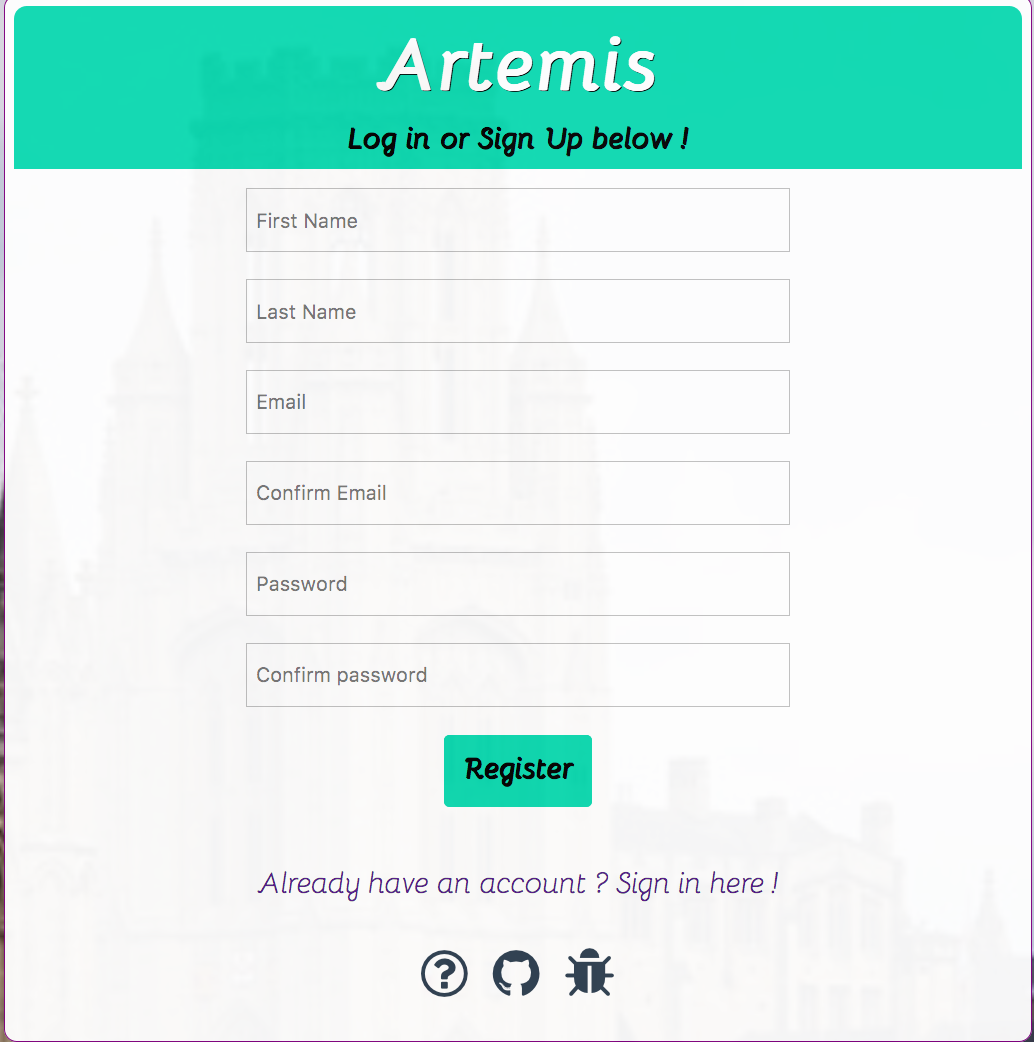
\includegraphics[scale=0.33]{chapters/appendices/figures/regForm.png}}
        \subfloat{ 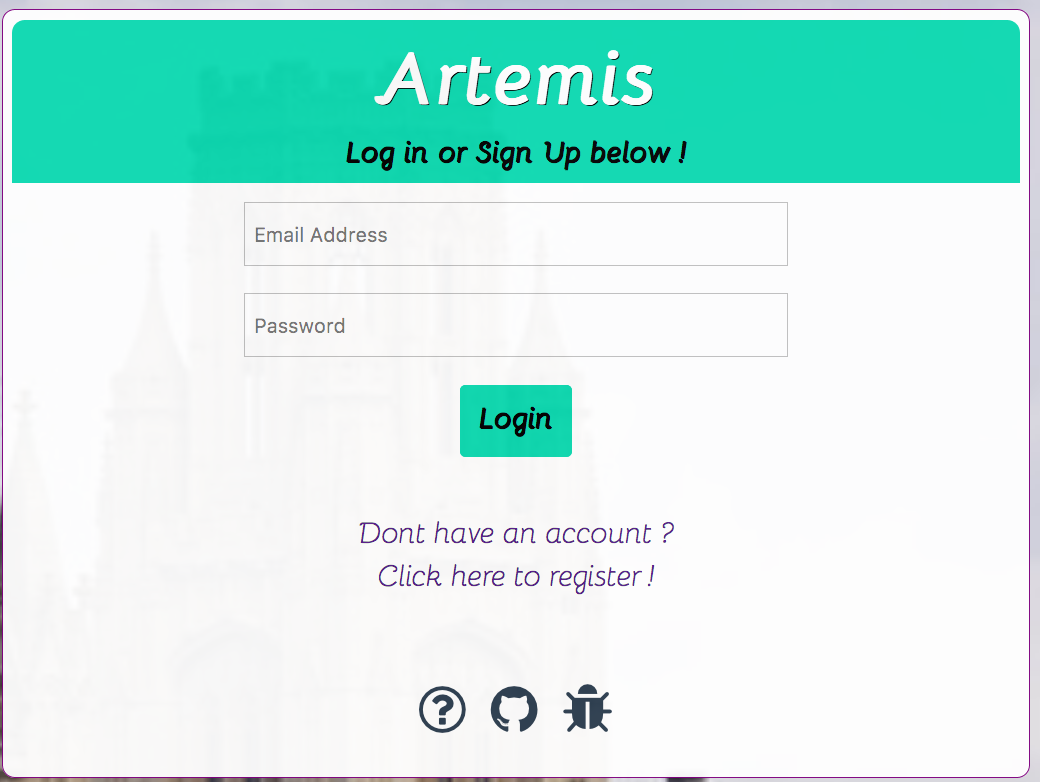
\includegraphics[scale=0.44]{chapters/appendices/figures/logInForm.png}}
        \caption[Log In and Registration Forms]{Log In and Registration Forms}
    \end{center}
\end{figure}

Whilst this creates a compact aesthetically pleasing UX for an able bodied user, an assistive device will almost certainly not be able to determine which form is hidden or not; It can be reasonably deduced that this makes the registration form inaccessible if not very hard to access for  visually impaired students \cite{Faulkner2012,MozillaDeveloperNetwork2017}. However this also easily remedied by the use of the \textit{aria-hidden} attribute which are dynamically updated via AJAX calls\cite{W3C2014a} when toggling the forms to effectively change the state of the relevant HTML elements\cite{Faulkner2012,W3C2014a} as illustrated below:

    \begin{figure}[h]
    	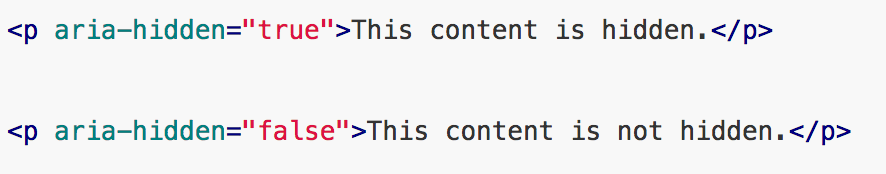
\includegraphics[scale=0.66,center]{chapters/appendices/figures/ariaHidden.png}
    	\mycaption[ARIA to Change State of HTML Element]{ARIA to Change State of HTML Element For Assistive Technology\cite{Faulkner2012}}
    	\label{ariaHidden}
    \end{figure}
    
    
\item\textbf{Validation, Notificaiton and Other Dynamically Generated Content}:

Artemis contains forms for the registration, login and user setting pages which are dynamically validated; generating error messages prompting users to make corrections in response to incorrect input. As is the norm with social networks Artemis generates notification e.g. If the user receives a message, notification or friend request. Artemis also has features such as an \textit{infinite scrolling newsfeed and personal} which generates content (i.e. posts) when a user scrolls down. All of this dynamically generated changes would be invisible to a screen reader, as assistive technology works best with static pages \cite{Sukardi2016}

In these cases a combination powerful ARIA live region features and appropriate role attributes can be used to enhance the ability of assisitve technology to detect dynamically generated content. The approach is explained as follows:
\begin{enumerate}
    \item \textit{Role}: As per the Data Role Model (Appendix \ref{fig:roleModelHTML}) features such as notifications and validation error prompts can be assigned the \textit{alert} role. This benefits assistive technology as  most modern browsers will send out a message to relevant technologies to inform their users \cite{MozillaDeveloperNetwork2017a} that an error message has been generated.
    \item \textit{Aria Live Regions}: Using the \textit{alert role} attribute alone is an aggressive strategy\cite{MozillaDeveloperNetwork2017a}, as a screen reader is forced to \textit{assertively} notify it\textquotesingle s user as soon as possible; deemed unnecessary and obtrusive in certain use cases for Artemis e.g. when generating lists for the purposes of live search results, message and notification drop down style interfaces (Figure \textbf{\ref{dropDown}}).

    
    \begin{figure}[H]
    \begin{center}
        \subfloat{ 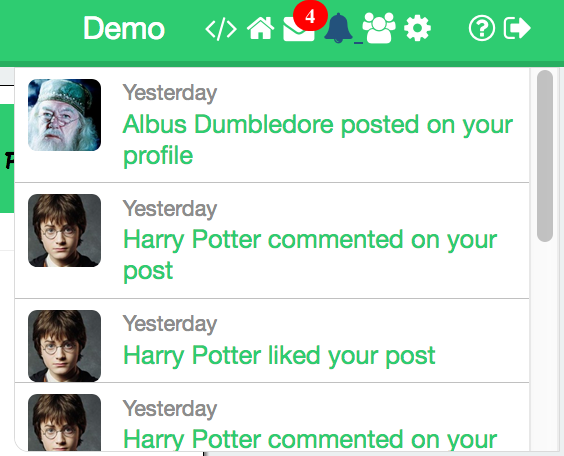
\includegraphics[scale=0.5]{chapters/appendices/figures/searchResults.png}}
        \subfloat{ 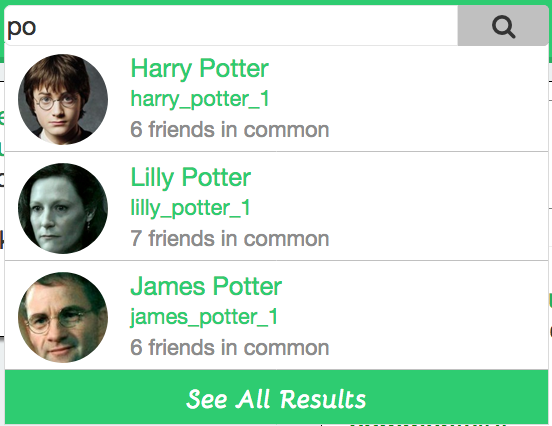
\includegraphics[scale=0.535]{chapters/appendices/figures/notificationResults.png}}
        \subfloat{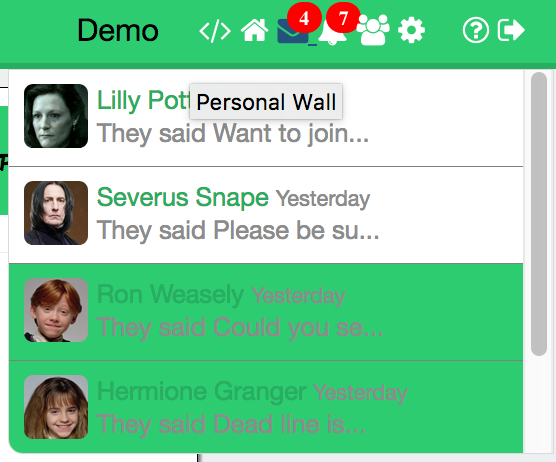
\includegraphics[scale=0.495]{chapters/appendices/figures/messageResults.png}}
        \caption[Drop Down Style Alerts - Not Ideal For Aggressive Strategy]{Drop Down Style Alerts - Not Ideal For Aggressive Strategy}
        \label{dropDown}
    \end{center}
    \end{figure}
    
    In these instances ARIA's Live Region features are particularly powerful at creating the desired UI semantics for dynamically generated features which are generated without a page reload \cite{MozillaDeveloperNetwork}. ARIA live features can be broken down into the following relevant features \cite{MozillaDeveloperNetwork} available to and implemented in Artemis:
    \begin{enumerate}
    \item \textit{aria-live}: This attribute can be used to change the \say{\textit{POLITENESS\_SETTING}}\cite{MozillaDeveloperNetwork} of a notification; with four available settings  \textit{off, assertive, polite and rude}. The \textit{assertive} and \textit{rude} settings are akin to assigning an \textit{alert} role to an HTML element, with the latter bearing the most similar semblance as it interrupts the UX to inform the client. The \textit{polite} setting is the one commonly opted for in Artemis for dynamically generated drop down list UI\textquotesingle s as it causes the assistive technology to alert the user the moment they are idle \cite{MicrosoftDeveloperNetwork}.
    
    \item \textit{aria-relevant}: This attribute has the following self explanatory options relevant to implementing Artemis; \textit{all, additions, removals}. These options are used to select relevant actions on constituent HTML elements of the live region of which assitive technology is to be informed 
    
    \item \textit{aria-atomic}: Setting this attribute to  a boolean \say{true} causes the entire live region to be treated as a single atomic entity to be traversed by assistive technology with every alert; it is turned off by default.
    
    \end{enumerate}

    Whilst live region features have been applied for various use cases in Artemis; The following implementation pattern has been adapted for the purposes of dynamically generated  lists in Artemis  as recommended by the MDN:
    
    \begin{figure}[h]
    	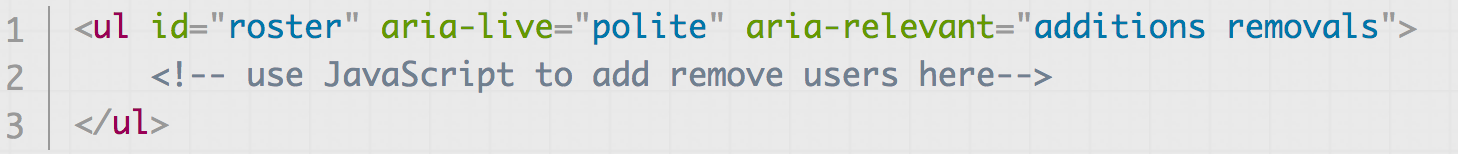
\includegraphics[scale=0.55,right]{chapters/appendices/figures/patternLive.png}
    	\mycaption[MDN Pattern for Accessible Dynamic Lists]{MDN Pattern for Accessible Dynamic Lists \cite{MozillaDeveloperNetwork}}
    	\label{ariaHidden}
    \end{figure}
    
    
    
\end{enumerate}
\end{enumerate}




\subsubsection{Creating Semantics}

As explained earlier ARIA has been used to create semantics for the complex or unconventional UI features of Artemis.This has been achieved by  using \textit{aria-labelledby, aria-describedby} and \textit{aria-label}, as per normative implementation patters prescribed by the MDN (vide WAI-ARIA), combined with roles compatible with the Data Role Model to override the native semantics of HTML elements so as to allow assistive technology to access the data as intended.

The aria-labelledby attribute contains element ids of it's constituent parent elements \cite{MozillaDeveloperNetworkb}, creating relationships between objects and their labels; aria-described by is very similar to the aforementioned except that it is used to supplement the relationship with an apt description \cite{MozillaDeveloperNetworkd}. As per the MDN, \say{\textit{a label describes \textbf{the essence} of an object, while \textbf{a description} provides more information that the user might need}}. The important thing to note is that without unique element id\textquotesingle s, corresponding relationship labels and descriptions where necessary a UI can become inaccessible in the case of the former or  hard to understand in the case of the latter \cite{MozillaDeveloperNetworkb,MozillaDeveloperNetworkd}.

The complexity of the UI in Artemis is best captured via the scope of a  single post; A complex relationship is visually implied between it's post body, sender's profile, time stamp, corresponding delete button, a list of comments (that is actually an iframe) on that post, like buttons etc; Coupled with being dynamically generated via a scrolling newsfeed/wall, from the perspective of an assistive technology an unrelated mess of HTML elements is generated.


To mitigate the problem of complex UI\textquotesingle s (both for the post feature and others) the following design pattern was adapted via MDN's list of normative implementations, for traversing nested HTML elements via their relationships:

    \begin{figure}[h]
    	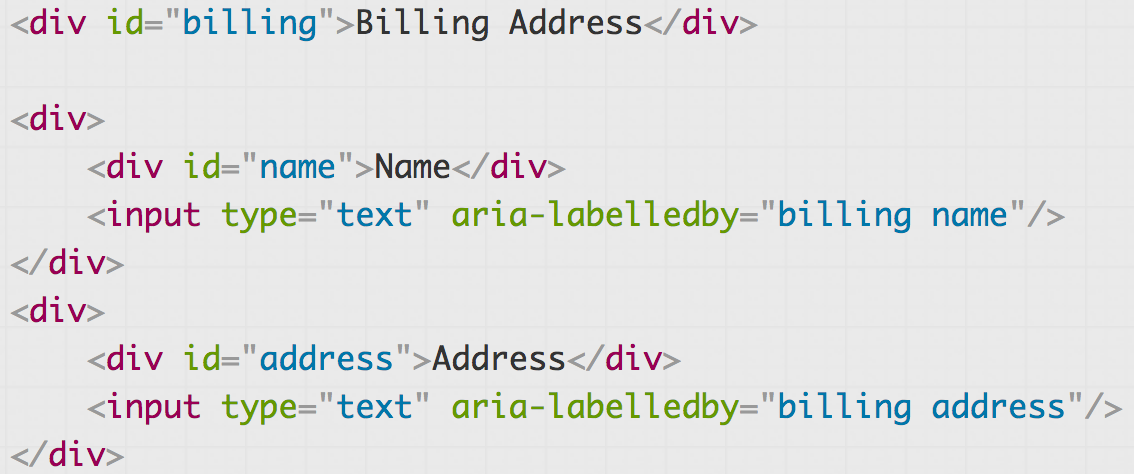
\includegraphics[scale=0.66,center]{chapters/appendices/figures/multipleLabel.png}
    	\mycaption[Multiple Labelling Strategy for Traversing Nested HTML Elements ]{ARIA to Change State of HTML Element For Assistive Technology\cite{MozillaDeveloperNetworkb}}
    \end{figure}

The above pattern was implemented by generating and concatenating unique ID tags to the HTML element and aria-labelledby attribute. Additionally these relationships were explained by the aria-described by feature \cite{MozillaDeveloperNetworkd}. Finally where deemed necessary native HTML element role semantics were overridden with applicable  normative roles as per the Data Role Model prescribed by WAI-ARIA; e.g. in the case of the comment\textquotesingle s iframe where a separate HTML page would confuse assistive technology so the roles have been overridden to depict a list element with constituent listitem elements.

The result of this strategy is clearly defined and described relationships between complex UI features, with semantically sensible HTML. Within the context of a single post, the user is able to navigate  individual semantic constituents of a post via unique ids, corresponding labels and supporting descriptions or roles; an approach adapted towards other UI features of Artemis as well.
